% XeLaTeX document
\documentclass[14pt,a4paper]{extarticle}
% \documentclass[14pt,a4paper]{article}


% Редактируем: конфигурация, личные настройки: имя, название предмета и пр. для титульной страницы и метаданных документа здесь
\newcommand{\university}{Национальный Исследовательский Ядерный Университет «МИФИ»}
\newcommand{\faculty}{Институт Ядерной Физики и Технологий}
\newcommand{\department}{Кафедра Теплофизики}
\newcommand{\city}{Москва}
\newcommand{\num}{ }
\newcommand{\docname}{Курсовой проект}
\newcommand{\subject}{Инженерные расчеты и проектирование реактора ВВЭР-1000}
\newcommand{\tutorname}{Ю. А. Маслов}
\newcommand{\studentname}{М. Д. Панин}
\newcommand{\group}{Б18-101}

% Не редактируем: используемые пакеты
% настройка кодировки, шрифтов и русского языка
\usepackage{fontspec}
\usepackage{polyglossia}
% рабочие ссылки в документе
\usepackage{hyperref}

% графика
\usepackage{graphicx}
\usepackage{tikz}

% поворот страницы
\usepackage{pdflscape}

\usepackage[euler]{textgreek}
% качественные листинги кода
\usepackage{minted}
\usepackage{listings}
\usepackage{lstfiracode}

% отключение копирования номеров строк из листинга, работает не во всех просмотрщиках (в Adobe Reader работает)
\usepackage{accsupp}
\newcommand\emptyaccsupp[1]{\BeginAccSupp{ActualText={}}#1\EndAccSupp{}}
\let\theHFancyVerbLine\theFancyVerbLine
\def\theFancyVerbLine{\rmfamily\tiny\emptyaccsupp{\arabic{FancyVerbLine}}}

% библиография
\bibliographystyle{templates/gost-numeric.bbx}
\usepackage{csquotes}
\usepackage[parentracker=true,backend=biber,hyperref=true,bibencoding=utf8,style=numeric-comp,language=auto,autolang=other,citestyle=gost-numeric,defernumbers=true,bibstyle=gost-numeric,sorting=ntvy]{biblatex}

% установка полей
\usepackage{geometry}

% нумерация картинок по секциям
\usepackage{chngcntr}

% дополнительные команды для таблиц
\usepackage{booktabs}

% для заголовков
\usepackage{caption}
\captionsetup[table]{position=top}
\usepackage{titlesec}
\usepackage[dotinlabels]{titletoc}

% разное для математики
\usepackage{amsmath, amsfonts,amsthm, mathtools}
%amssymb
\usepackage{unicode-math}
% водяной знак на документе, см. main.tex
\usepackage[printwatermark]{xwatermark}

\usepackage{environ}         % provides \BODY
\usepackage{etoolbox}        % provides \ifdimcomp
\usepackage{graphicx}        % provides \resizebox
\usepackage{resizegather}

% Не редактируем: параметры используемых пакетов и не только
% настройки polyglossia
\setdefaultlanguage{russian}
\setotherlanguage{english}

% локализация
\addto\captionsrussian{
	\renewcommand{\figurename}{Рисунок}%
	\renewcommand{\partname}{Глава}
	\renewcommand{\contentsname}{\centerline{Содержание}}
	\renewcommand{\listingscaption}{Листинг}
}

% основной шрифт документа
\setmainfont{Liberation Serif}
\newfontfamily\cyrillicfont{Liberation Serif}[Script=Cyrillic]

% перечень использованных источников
\addbibresource{refs.bib}

% настройка полей
\geometry{top=2cm}
\geometry{bottom=2cm}
\geometry{left=2cm}
\geometry{right=2cm}
\geometry{bindingoffset=0cm}

% настройка ссылок и метаданных документа
\hypersetup{unicode=true,colorlinks=true,linkcolor=blue,citecolor=green,filecolor=magenta,urlcolor=cyan,
	pdftitle={\docname},
	pdfauthor={\studentname},
	pdfsubject={\subject},
	pdfcreator={\studentname},
	pdfproducer={Overleaf},
	pdfkeywords={\subject}
}

% настройка подсветки кода и окружения для листингов
\usemintedstyle{colorful}
\newenvironment{code}{\captionsetup{type=listing}}{}

% шрифт для листингов с лигатурами
\setmonofont{FiraCode-Regular.otf}[
	SizeFeatures={Size=10},
	Path = templates/,
	Contextuals=Alternate
]

% оформления подписи рисунка
\captionsetup[figure]{labelsep = period}

% подпись таблицы
% \DeclareCaptionFormat{hfillstart}{\hfill#1#2#3\par}
% \captionsetup[table]{format=hfillstart,labelsep=newline,justification=centering,skip=-10pt,textfont=bf}

% путь к каталогу с рисунками
\graphicspath{{fig/}}

% Внесение titlepage в учёт счётчика страниц
\makeatletter
\renewenvironment{titlepage} {
	\thispagestyle{empty}
}
\makeatother

\counterwithin{figure}{section}
\counterwithin{table}{section}

\titlelabel{\thetitle.\quad}

% для удобного конспектирования математики
\mathtoolsset{showonlyrefs=false}
\theoremstyle{plain}
\newtheorem{theorem}{Теорема}[section]
\newtheorem{proposition}[theorem]{Утверждение}
\theoremstyle{definition}
\newtheorem{corollary}{Следствие}[theorem]
\newtheorem{problem}{Задача}[section]
\theoremstyle{remark}
\newtheorem*{nonum}{Решение}

% настоящее матожидание
\newcommand{\MExpect}{\mathsf{M}}

% объявили оператор!
\DeclareMathOperator{\sgn}{\mathop{sgn}}

% перенос знаков в формулах (по Львовскому)
\newcommand*{\hm}[1]{#1\nobreak\discretionary{} {\hbox{$\mathsurround=0pt #1$}}{}}


% \numberwithin{equation}{section}equation

\newlength{\myl}
\let\origequation=\equation
\let\origendequation=\endequation

\DeclareSymbolFont{lettersA}{U}{txmia}{m}{it} 
\SetSymbolFont{lettersA}{bold}{U}{txmia}{bx}{it} 
\DeclareFontSubstitution{U}{txmia}{m}{it} 
\DeclareSymbolFontAlphabet{\mathfrak}{lettersA}

\DeclareMathSymbol{\alphaup}{\mathord}{lettersA}{11}
\DeclareMathSymbol{\betaup}{\mathord}{lettersA}{12}
\DeclareMathSymbol{\gammaup}{\mathord}{lettersA}{13}
\DeclareMathSymbol{\deltaup}{\mathord}{lettersA}{14}
\DeclareMathSymbol{\epsilonup}{\mathord}{lettersA}{15}
\DeclareMathSymbol{\zetaup}{\mathord}{lettersA}{16}
\DeclareMathSymbol{\etaup}{\mathord}{lettersA}{17}
\DeclareMathSymbol{\thetaup}{\mathord}{lettersA}{18}
\DeclareMathSymbol{\iotaup}{\mathord}{lettersA}{19}
\DeclareMathSymbol{\kappaup}{\mathord}{lettersA}{20}
\DeclareMathSymbol{\lambdaup}{\mathord}{lettersA}{21}
\DeclareMathSymbol{\muup}{\mathord}{lettersA}{22}
\DeclareMathSymbol{\nuup}{\mathord}{lettersA}{23}
\DeclareMathSymbol{\xiup}{\mathord}{lettersA}{24}
\DeclareMathSymbol{\piup}{\mathord}{lettersA}{25}
\DeclareMathSymbol{\rhoup}{\mathord}{lettersA}{26}
\DeclareMathSymbol{\sigmaup}{\mathord}{lettersA}{27}
\DeclareMathSymbol{\tauup}{\mathord}{lettersA}{28}
\DeclareMathSymbol{\upsilonup}{\mathord}{lettersA}{29}
\DeclareMathSymbol{\phiup}{\mathord}{lettersA}{30}
\DeclareMathSymbol{\chiup}{\mathord}{lettersA}{31}
\DeclareMathSymbol{\psiup}{\mathord}{lettersA}{32}
\DeclareMathSymbol{\omegaup}{\mathord}{lettersA}{33}
\DeclareMathSymbol{\varepsilonup}{\mathord}{lettersA}{34}
\DeclareMathSymbol{\varthetaup}{\mathord}{lettersA}{35}
\DeclareMathSymbol{\varpiup}{\mathord}{lettersA}{36}
\DeclareMathSymbol{\varrhoup}{\mathord}{lettersA}{37}
\DeclareMathSymbol{\varsigmaup}{\mathord}{lettersA}{38}
\DeclareMathSymbol{\varphiup}{\mathord}{lettersA}{39}

\renewcommand{\alpha}{\alphaup}
\renewcommand{\beta}{\betaup}
\renewcommand{\gamma}{\gammaup}
\renewcommand{\delta}{\deltaup}
\renewcommand{\epsilon}{\varepsilonup}
\renewcommand{\zeta}{\zetaup}
\renewcommand{\eta}{\etaup}
\renewcommand{\theta}{\theteaup}
\renewcommand{\iota}{\iotaup}
\renewcommand{\kappa}{\kappaup}
\renewcommand{\lambda}{\lambdaup}
\renewcommand{\mu}{\muup}
\renewcommand{\nu}{\nuup}
\renewcommand{\xi}{\xiup}
\renewcommand{\pi}{\piup}
\renewcommand{\rho}{\rhoup}
\renewcommand{\sigma}{\sigmaup}
\renewcommand{\tau}{\tauup}
\renewcommand{\upsilon}{\upsilonup}
\renewcommand{\phi}{\varphiup}
\renewcommand{\chi}{\chiup}
\renewcommand{\omega}{\omegaup}
\renewcommand{\vartheta}{\varthetaup}
\renewcommand{\varpi}{\varpiup}
\renewcommand{\varrho}{\varrhoup}
\renewcommand{\varsigma}{\varsigmaup}
\renewcommand{\varepsilon}{\varepsilonup}
\renewcommand{\varphi}{\varphiup}

% водяной знак для обозначения статуса документа
% \newwatermark[allpages,color=red!5,angle=45,scale=3,xpos=0,ypos=0]{DRAFT}
\begin{document}
\begin{titlepage}	% начало титульной страницы

	\begin{center}		% выравнивание по центру
		Министерство Науки и Высшего Образования Российской Федерации\\ 
		\footnotesize Федеральное Государственное Автономное Образовательное Учреждение Высшего Образования\\  
		\large \textbf{\university} \\[0.5cm]
		\faculty \\[0.25cm]
		\department \\[2cm]
		% название института, затем отступ 6см

		\LARGE \textbf{Пояснительная записка\\ к курсовому проекту на тему:}
 \\[0.5cm] % название работы, затем отступ 0,5см
		\Large «Инженерные расчеты и проектирование реактора ВВЭР-1000» \num \\[2cm]
\normalsize		% \large Тема работы\\[5cm]
\begin{minipage}[b]{0.4\textwidth}
\raggedright
Студент: \\[1cm]
Руководитель: \\[0.5cm]
Руководитель\\ со стороны 5 кафедры: \\[1cm]
Рецензент \\[1cm]
Зав. Кафедрой \\
\end{minipage}%
\begin{minipage}[b]{0.3\textwidth}
\raggedright
Панин М.Д. \\[1cm]
Маслов Ю.А. \\[0.5cm]
Терновых М.Ю. \\ \  \\[1cm]
\  \\[1cm]
Харитонов В.С.\\
\end{minipage}%
\begin{minipage}[b]{0.3\textwidth}
\raggedright
\hrulefill\\[1cm]
\hrulefill\\[0.5cm]
\ \\ \hrulefill\\[1cm]
\hrulefill\\[1cm]
\hrulefill\\
\end{minipage}
\end{center}


	\vfill % заполнить всё доступное ниже пространство

	\begin{center}
		\large \city \\
		\large \the\year % вывести дату
	\end{center} % закончить выравнивание по центру

\end{titlepage} % конец титульной страницы

\vfill % заполнить всё доступное ниже пространство

\section*{СПИСОК ОБОЗНАЧЕНИЙ И СОКРАЩЕНИЙ}
\addcontentsline{toc}{section}{\protect СПИСОК ОБОЗНАЧЕНИЙ И СОКРАЩЕНИЙ}%
% \subsection*{Сокращения}
\noindent ВКР – выпускная квалификационная работа

\noindent РУ — реакторная установка

\noindent ЯЭУ — ядерная энергетическая установка

\noindent ГЦН — главный циркуляционный насос

\noindent АЗ — активная зона

\noindent ТВС — тепловыделяющая сборка

\noindent КПД — коэффициент полезного действия

\noindent СУЗ — стержни управления защитой

\noindent АЭС — атомная энергетическая станция
% \subsection*{Обозначения}


\section*{РЕФЕРАТ}
% \addcontentsline{toc}{section}{\protect РЕФЕРАТ}%
Выпускная квалификационная работа содержит 61 - страниц, 55 - рисунков, 11 - таблиц и 9 -источников.

РЕАКТОР ВВЭР-1000, АКТИВНАЯ ЗОНА, ГИДРОДИНАМИКА, ТЕПЛООБМЕН, ОТКЛЮЧЕНИЕ ГЦН, ПОВЫШЕНИЕ МОЩНОСТИ,  МОДЕЛИРОВАНИЕ, ПРОГРАММНЫЙ МОДУЛЬ ТРЕТОН

В работе выполнено моделирование теплогидравлических параметров активной зоны ВВЭР-1000 в номинальном режиме, а так же в не номинальных режимах с увеличением мощности реактора, и с отключением одного из четырех и двух их четырех ГЦН.
\begin{enumerate}
    \item В первой главе приведен обзор конструкции и предоставлена общая информация реакторной установки ВВЭР-1000
    \item Во второй главе осуществлен теплофизический расчет реактора ВВЭР-1000 в номинальном режиме
    \item В третий главе осуществлен теплофизический расчет ВВЭР-1000 на программном модуле ТРЕТОН в номинальном режиме, а так же сравнения данных с аналитическим расчетом, осуществлен расчет в неноминальных режимах с увеличением мощности на 105\%, 110\%, 115\% и отключением одного и двух стоящих друг на против друга ГЦН. 
\end{enumerate}

% Не редактируем: Страница содержания (формируется автоматически из section, subsection и пр., указанных в content.tex)
\include{templates/tocpage}
\section*{ВВЕДЕНИЕ}
\addcontentsline{toc}{section}{\protect ВВЕДЕНИЕ}
В настоящее время в атомной промышленности большое распространение имеют водо-водяные корпусные реакторы, как кипящие (американские PWR), так и некипящие (русские ВВЭР). Благодаря использованию воды в качестве теплоносителя и замедлителя такие установки относительно дешевые в эксплуатации и достаточно безопасные ввиду возможности обеспечения отрицательного коэффициента реактивности. Отдельно стоит отметить установку ВВЭР-1000, имеющую наибольшее распространение среди реакторов такой серии (37 действующих установок из 60-и ВВЭР). Проект хорошо себя зарекомендовал и находится в эксплуатации с 1980 года, когда был установлен первый реактор такого типа на пятом энергоблоке Нововоронежской АЭС, новые установки данной модели производятся по сей день. При строительстве первых реакторов ВВЭР-1000 проектом закладывлся срок эксплуатации в 30 лет, сейчас же учитывая современные научные знания срок службы таких установок и идентичных новых был увеличен до 60 лет. При столь длинных сроках эксплуатации, на которые рассчитаны РУ ВВЭР-1000 возникает потребность адаптировать существующие к современным энергетическим потребностям. 

Проектом такие РУ изначально рассчитывались на большую мощность, что позволяет по необходимости эффективнее утилизировать мощностные ресурсы установки, благодаря чему можно сэкономить на строительстве новых энергоблоков. Так, например, на балаковской АЭС для ВВЭР-1000 серийного проекта В-320 успешно было проведено мероприятие по повышению мощности на 4\% \cite{104балаково}. 

Таким образом проблема вертикального масштабирования по мощности наиболее актуальна для реакторов типа ВВЭР-1000, что определяет и \textit{актуальность} данной работы. 

\textit{Целью} данной работы являлось расчет и исследования температурных полей реакторной установки ВВЭР-1000 при работе на повышенной мощности, а также на пониженной при отключении одного из четырех и двух из четырех ГЦН. \textit{Практическая значимость} данной работы состоит в определении максимальных температур и выводов о работоспособности РУ в исследуемых режимах работы. На основе поставленной цели были сформированы следующие задачи:
\begin{itemize}
    \item Произвести теплофизический и нейтронно-физический расчет ВВЭР-1000 и определить характеристики РУ в номинальном режиме работы 
    \item Ознакомится с расчетной моделью программного комплекса ТРЕТОН и прозвести валидационный расчет РУ в номинальном режиме.
    \item Произвести рассчетное исследование работы реактора в режиме повышенной мощности, определить максимальные температуры и их превышения и сделать вывод о возможности работы реактора в таком режиме
    \item Произвести рассчетное исследование работы реактора при отключении одного из трех и двух из трех, произвести анализ температурных полей и сделать вывод о возможности работы РУ при пониженной мощности
\end{itemize}

% \section*{Введение}
% \addcontentsline{toc}{section}{\protect Введение}%
% IN PROGRESS...

% \RenewEnviron{equation}{
%   \settowidth{\myl}{$\BODY$}                       % calculate width and save as \myl
%   \origequation
%   \ifdimcomp{\the\linewidth}{>}{\the\myl}
%   {\ensuremath{\BODY}}                             % True
%   {\resizebox{\linewidth}{!}{\ensuremath{\BODY}}}  % False
%   \origendequation
% }


\section{Описание конструкции реактора}
ВВЭР-1000 конструктивно относится к классу гетерогенных корпусных реакторов. С точки зрения спектра нейтронов он является тепловым. В качестве теплоносителя и замедлителя используется легкая вода под давлением. В качестве топлива в реакторе используется низкообогащенным диоксид урана $UO_2$. Общий вид реактора в сборке представлен на рисунке \ref{pic:scheme}. 


В верхней части реактора расположена герметично закрытая крышка с установленными на ней приводами механизмов и органов регулирования и защиты. Также крышка оснащена патрубками для вывода кабелей датчиков внутриреакторного контроля. Крепление  к корпусу осуществляется с помощью шпилек. 


Реактор имеет двухконтурную систему. Энергия, выделяющаяся в результате ценой реакции деления ядер урана, преобразуется в тепловую энергию теплоносителя первого контура. Далее нагретый теплоноситель поступает с помощью тепловых насосов в парогенераторы, где происходит отдача тепла воде второго контура. Образовавшийся в парогенераторах пар далее поступает в паротурбинную установку, приводящую в движение турбогенератор, который вырабатывает электроэнергию.
% 
После передачи энергии в парогенераторах вода первого контура поступает в реактор через нижний ряд напорных патрубков. Сплошная кольцевая перегородка между рядами нижних и верхних патрубков, дистанцирующая корпус реактора и его шахту, формирует движение потока теплоносителя вниз. Поэтому вода проходит вниз по кольцевому зазору между корпусом и внутрикорпусной шахтой, затем через перфорированное эллиптическое днище и опорные трубы шахты входит в топливные тепловыделяющие сборки. Из ТВС через перфорированную нижнюю плиту блока защитных труб (БЗТ) теплоноситель выходит в межтрубное пространство БЗТ, а затем через кольцевой зазор между шахтой и корпусом и четыре верхних выходных патрубка из реактора.

%Параграф про водо-водянистость
%Параграф про корпусность
%Параграф про двухконтурность
%
\noindent
\begin{minipage}[t]{.5\textwidth}
\raggedright
\cite{лескин2011физические}
\begin{figure}[H]
	\begin{center}
		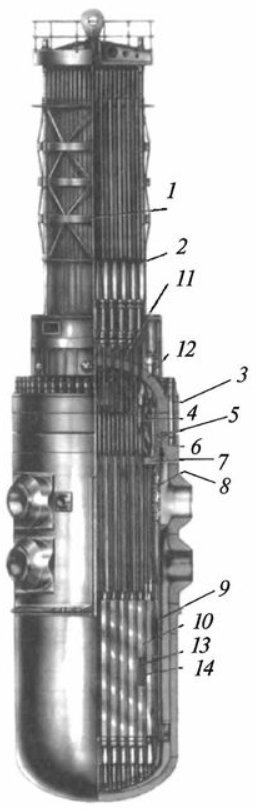
\includegraphics[scale=0.7]{Scheme.png}
		\caption{\small Общий вид реактора ВВЭР-1000 в сборе }
		\label{pic:scheme} % название для ссылок внутри кода
	\end{center}
\end{figure}
%
\end{minipage}%    <---------------- Note the use of "%"
\begin{minipage}[t]{.5\textwidth}
\raggedright
\begin{enumerate}
\item верхний блок; 
\item привод СУЗ;
\item шпилька;
\item труба для загрузки образцов-свидетелей;
\item уплотнение;
\item корпус реактора;
\item блок защитных труб;
\item шахта;
\item выгородка активной зоны;
\item топливные сборки;
\item теплоизоляция реактора; 
\item крышка реактора;
\item регулирующие стержни;
\item топливные стержни.
\end{enumerate}
\end{minipage}

\section{Теплофизический расчет}

\subsection{Постановка задачи}
В данном разделе будут определены основные термодинамические и гидравлические параметры реакторной установки. Теплофизический расчет подразумевает следующий ряд задач:

    \begin{enumerate}
        \item Выбор турбины и разработка принципиальной теплосиловой схемы установки;
        \item Рассчет КПД проектируемой установки;
        \item Рассчет основных теплофизических характеристик, таких как мощность ТВС и твэла, расход и скорость теплоносителя, коэффициент теплоотдачи;
        \item Построение распределения температур теплоносителя, оболочки и топлива по длинне для наиболее напряжённого канала; 
        \item Определение максимально возможных температур теплоносителя, оболочки и топлива;
        \item Рассчёт перепадов давлений и мощности, необходимой на прокачку теплоносителя;
        \item Рассчёт коэффициента запаса до кризиса теплообмена;
    \end{enumerate}

\subsection{Исходные данные для проведения расчетов}


Для проведения теплогидравлического расчета реакторной установки использовались следующие характеристики, представленные в Таблице \ref{tabular:data}.

\begin{table}[H]
	\caption{Исходные данные для проектируемого РУ ВВЭР-1000}
	\begin{center}
        \begin{tabular}{|l|c|}
        \toprule
         Характеристика & Значение \\ 
         \midrule
         \hline
         Электрическая мощность реактора, МВт & 1000 \\
         \hline\ 
         Температура теплоносителя на входе в АЗ $T_{\text{вх}}$, $^\circ C$  & 287 \\ 
         \hline\
         Температура теплоносителя на выходе АЗ $T_{\text{вых}}$, $^\circ C$ & 320 \\ 
         \hline
         Температура питательной воды, , $^\circ C$ & 220 \\ 
         \hline
         Температура свежего пара, $^\circ C$  &  274.6 \\ 
         \hline
         Давление свежего пара & 5.9 \\ 
         \hline
         Температура пара после пароперегревателей, $^○C$ & 250 \\ 
         \hline
         Давление в АЗ, МПа & 15.7 \\ 
         \hline
         Степень сухости пара после ЦВД и ЦНД, \% & 80 \\ 
         \hline
         Количество петель РУ & 4 \\ 
         \hline
         Число ТВС $N_{\text{ТВС}}$, шт  & 163 \\ 
         \hline
         Число твэл в ТВС $N_{\text{твэл}}$, шт & 317 \\ 
         \hline
         Коэффициент неравномерности по высоте АЗ  & 1.5 \\ 
         \hline
         Коэффициент неравномерности по радиусу АЗ & 1.25 \\ 
         \hline
         Высота АЗ $H_{\text{AZ}}$, м & 3.5 \\ 
         \hline
         Диаметр твэл $d_{\text{тв}}$, мм & 9.1 \\ 
         \hline
         Размер ТВС «под ключ» $a$, мм & 234 \\ 
         \hline
         Толщина чехла ТВС $\delta_{\text{чехла}}$, мм & 1.5 \\
         \hline
         Диаметр центрального канала в ТВС $D_{\text{ц.к}}$, мм & 10.3 \\ 
         \hline
         Число направляющих каналов в ТВС $N_{\text{н.к.}}$, шт & 12 \\ 
         \hline
         Шаг решетки ТВС $S_m$, мм & 12,75 \\ 
         \hline
         Диаметр направляющего канала в ТВС $D_{\text{н.к}}$, мм & 12.6 \\ 
         \hline
         Толщина оболочки твэл $\delta_{\text{твэл}}$, мм & 0.65 \\ 
         \hline
         Толщина газового зазора в твэл $\delta_{\text{г}}$, мм & 0.135 \\ 
         \hline
         Диаметр топливной таблетки $d_{\text{топ}}$, мм. & 7.53 \\ 
         \hline
         Диаметр отверстия топливной таблетки $d_{\text{\text{отв}}}$, мм & 1.3 \\ 
        %  \hline
        %  Число СУЗ $N_{\text{СУЗ}}$, шт & 109 \\ %сомнительная штука https://ru.wikipedia.org/wiki/%D0%92%D0%92%D0%AD%D0%A0-1000
        %  \hline
        %  Диаметр СУЗ $D_{\text{СУЗ}}$, мм & 8.2 \\
         \bottomrule
		\end{tabular}
		\label{tabular:data}
	\end{center}
\end{table}




\subsection{Выбор турбины}
В качестве турбины в расчетах будем использовать модель К-1000-60/1500-2. Её характеристики представлены в таблице \ref{tabular:turbine}

\cite{Андрушечко}
\begin{table}[H]
	\caption{Параметры турбины К-1000-60/1500-2 }
	\begin{center}
        \begin{tabular}{|l|c|}
        \toprule
         Параметр & Значение или Название \\ 
         \midrule
         \hline
         Прототип турбины &  К-1000-60/1500\\ 
         \hline
         Температура питательной воды, $^\circ C$ & 220 \\ 
         \hline
         Температура свежего пара, $^\circ C$  & 274.6\\
         \hline
         Давление свежего пара, $^\circ C$ & 5.9 \\ 
         \hline
         Температура после промежуточного перегрева, $^○C$ & 250 \\ 
         \hline
         Количество регенеративных подогревателей & 7 \\ 
         \bottomrule
		\end{tabular}
		\label{tabular:turbine}
	\end{center}
\end{table}


\begin{figure}[H]
	\begin{center}
		\includegraphics[scale=0.5]{teploscheme.jpg}
		\caption{Тепловая схема АЭС: 1 – ядерный реактор, 2 – главный
циркуляционный насос, 3 – парогенератор, 4 – цилиндр высокого давления, 5 –
сепаратор-пароперегреватель, 6 – цилиндры низкого давления, 7 – генератор, 8
– конденсатор, 9 – конденсационный электронасос, 10 – подогреватель низкого
давления, 11 – охладитель, 12 – станция насосная, 13 – деаэратор, 14 –
плунжерный электронасос, 15 – подогреватель высокого давления, 16 –
конденсационный насос с гидротурбинным приводом}
		\label{pic:teplocheme} % название для ссылок внутри кода
	\end{center}
\end{figure}


\subsection{Расчет КПД термодинамического цикла}


\begin{figure}[H]
	\begin{center}
		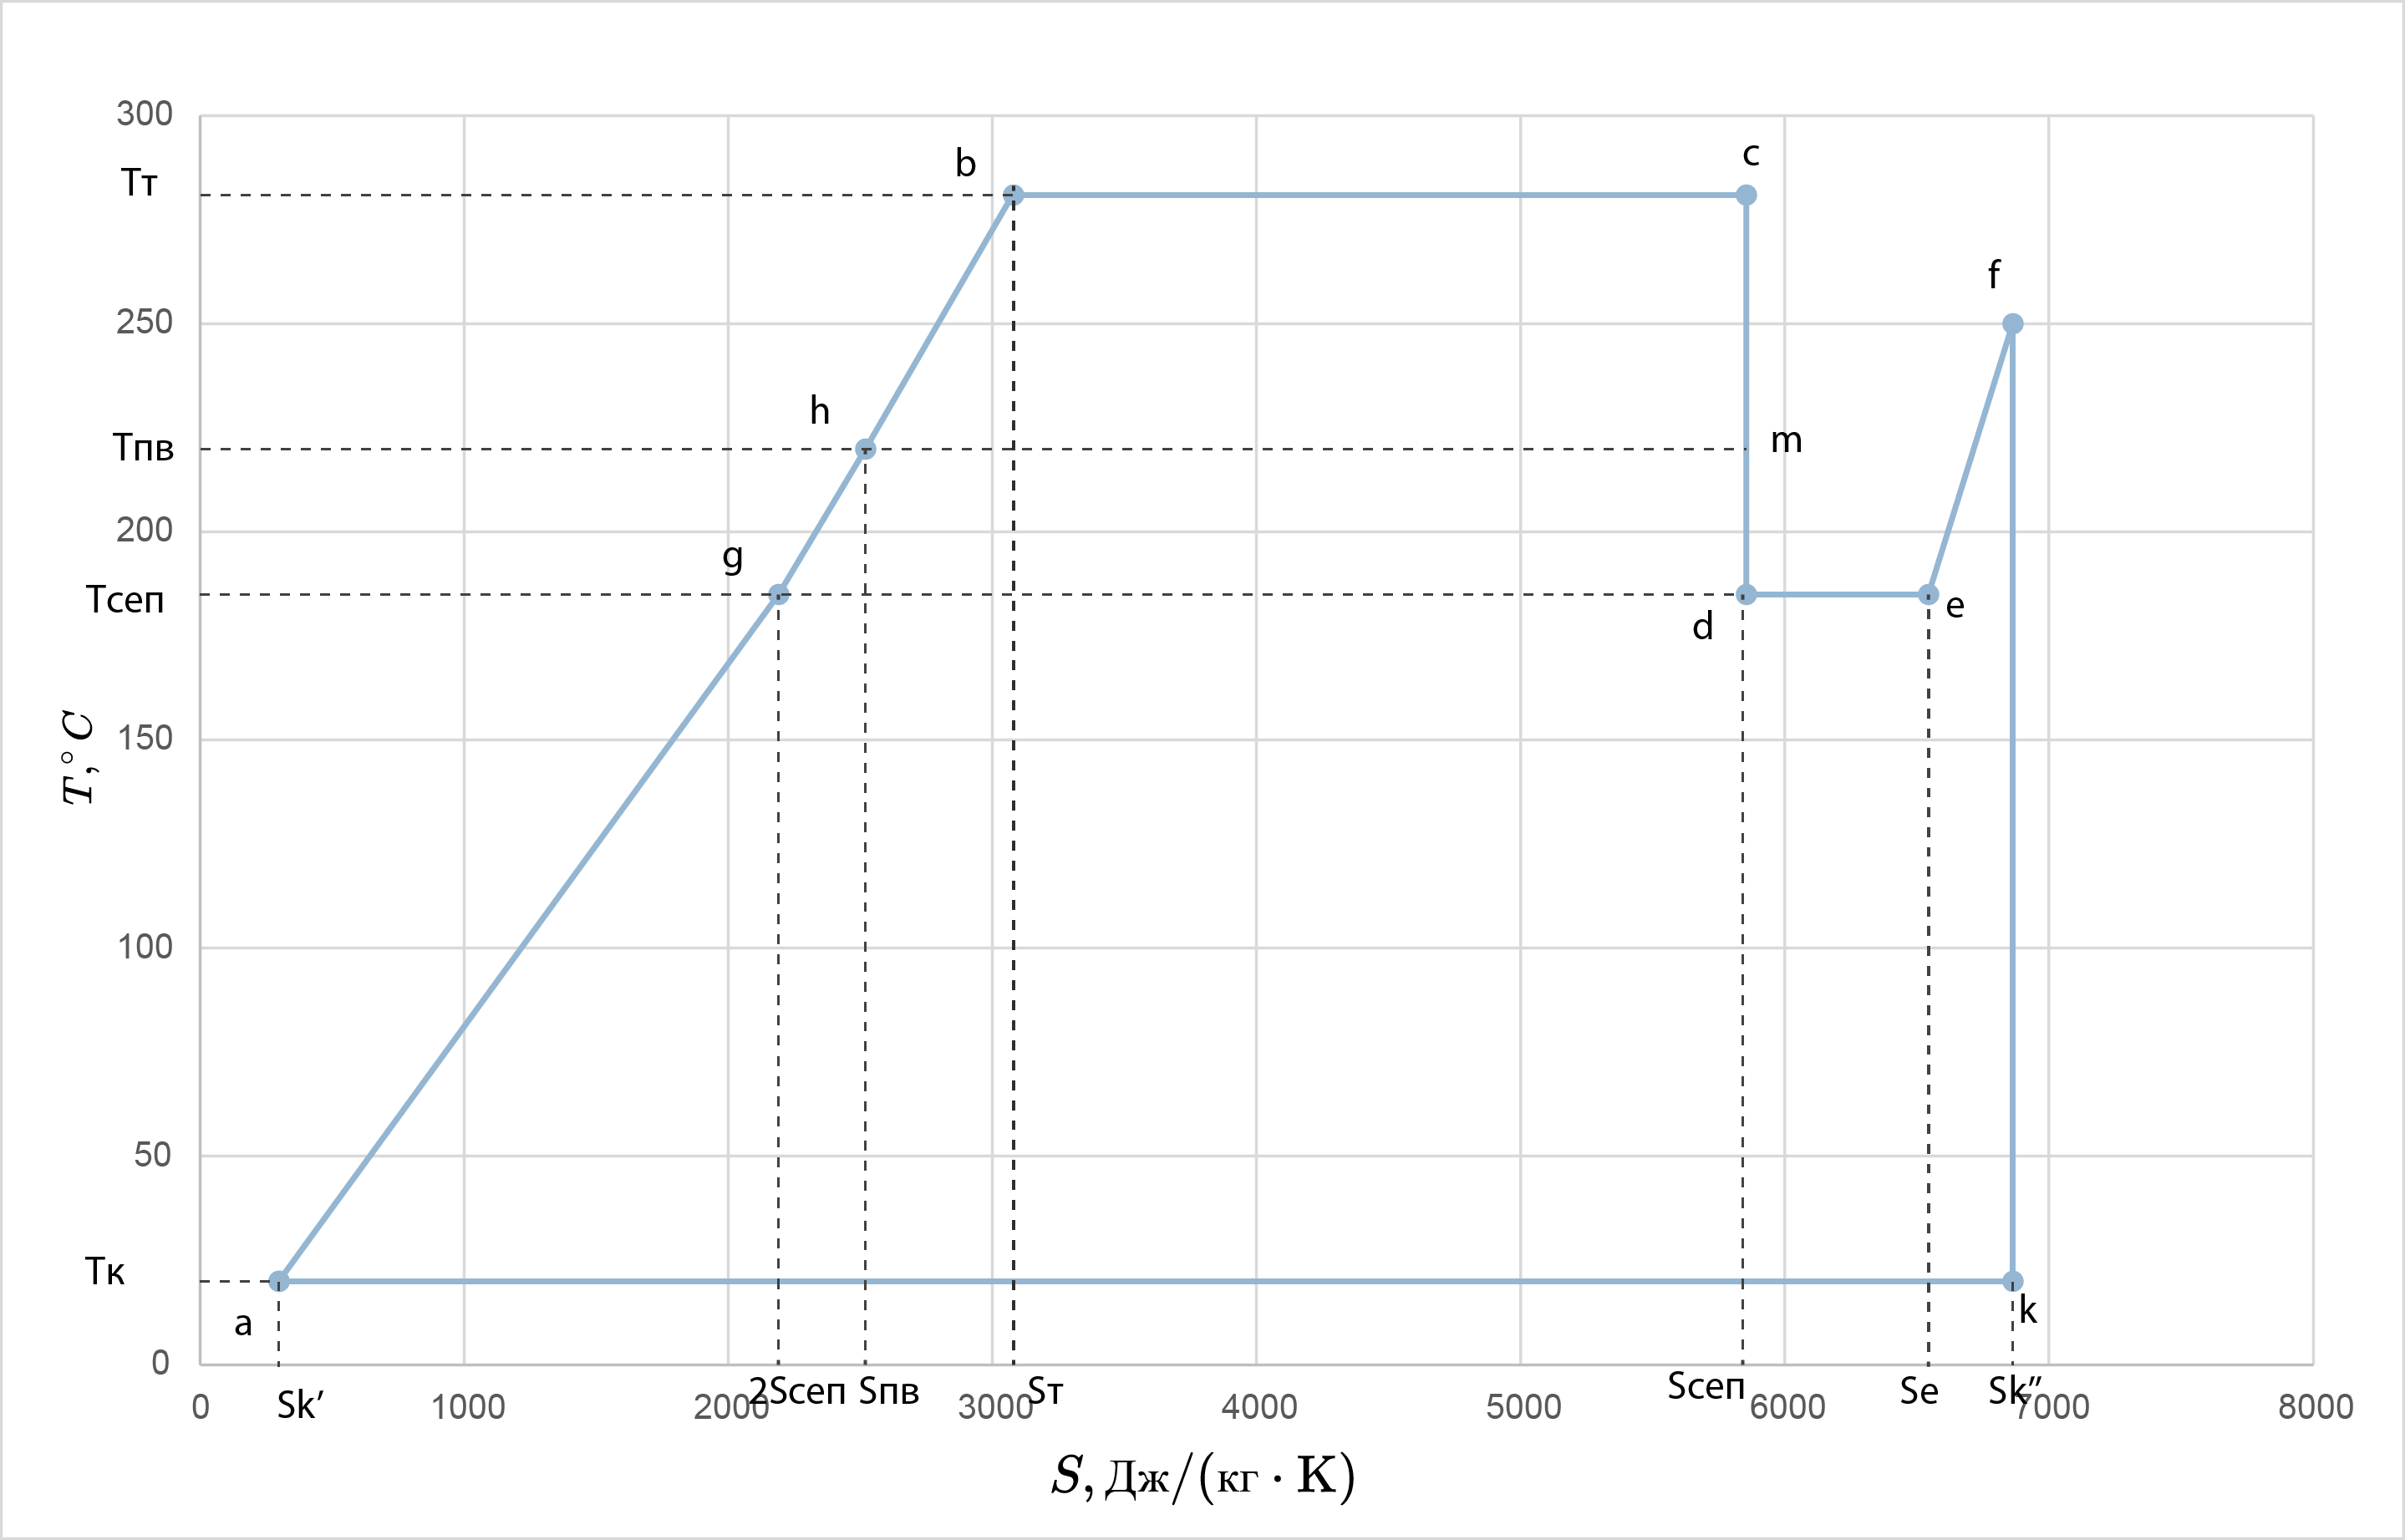
\includegraphics[scale=0.17]{TS.png}
		\caption{ T­S диаграмма турбинного цикла в реакторе ВВЭР­-1000 : hbc — нагрев и испарение в парогенераторе; cd — расширение пара в ЦВД; de — пар отделяется от конденсата в сепараторе; ef — пар поступает в промежуточный пароперегреватель; fk — расширение пара в ЦНД; ka — конденсация в конден­саторе; ag — регенеративный подогрев в ПНД; gh — регенеративный подогрев в ПВД;
        }
		\label{pic:TS} % название для ссылок внутри кода
	\end{center}
\end{figure}

\begin{table}[H]
	\caption{Значения параметров TS-диаграммы}
	\begin{center}
        \begin{tabular}{|c|c|c|c|c|}
        \toprule
         Точка & P, МПа & T, $^\circ C$ & S, Дж/(кг $\cdot$ К) & h, кДж/кг \\ 
         \midrule
         \hline
          h & 5.9 & 220 & 2516.4 & 942.9\\ 
         \hline
          b & 5.9 & 274.6 & 3017.4 & 1208.1 \\ 
         \hline
          c & 5.9 & 274.6 & 5898.01 & 2785.6\\ 
         \hline
          d & 0.98 & 179.189 & 5898.01 & 2462.7 \\ 
         \hline
          e & 0.98 & 179.189 & 6591.7 & 2776.4 \\ 
         \hline
          f & 0.98 & 250  & 6936.1 & 2943.61 \\ 
         \hline
          k & 0.004 & 28.7 & 6936.1 & 2099.5 \\ 
         \hline
          k′ & 0.004 & 28.7 & 416.66 & 119.656 \\ 
         \hline
          a & 5.9  & 28.7 & 414.9 & 125.1 \\ 
         \hline
          g & 0.98 & 179.2 & 2130.2 & 758.9 \\ 
         \bottomrule
		\end{tabular}
		\label{tabular:coeffs}
	\end{center}
\end{table}

Произведём расчет КПД для турбины К-1000-60/1500. Термический КПД без регенерации \cite{КирилловСправочник}:
\begin{equation}
\texteta_{t0}=1 - 
\frac{T_{k} ⋅ \left( s_{f} - s_{a} \right) ⋅ x_{d}}
{\left( h_{c} - h_{g} \right) +x_{d}\left( \left( h_{g} - h_{a} \right) + \left( h_{f} - h_{e} \right) \right)}
\end{equation}
\begin{equation}
\eta_{t0} = 
1 - 
\frac{3.017 \cdot 10^{ 2 } ⋅ \left( 6.936 \cdot 10^{ 3 } - 4.149 \cdot 10^{ 2 } \right) ⋅ 8.445 \cdot 10^{ -01 }}
{\left( 2.786 \cdot 10^{ 6 } - 7.589 \cdot 10^{ 5 } \right) + 8.445 \cdot 10^{ -01 } \left( \left( 7.589 \cdot 10^{ 5 } - 1.250 \cdot 10^{ 5 } \right) + \left( 2.944 \cdot 10^{ 6 } - 2.776 \cdot 10^{ 6 } \right) \right)}
\end{equation}
\begin{equation}
\eta_{t0}=3.854 \cdot 10^{ -01 }
\end{equation}

Термический КПД с идеальной регенерацией:

\begin{equation}
η_{t∞}=1 -
\frac{T_{k} ⋅ \left( s_{f} - s_{g} \right) \left( s_{c} - s_{h} \right)}
{\left(h_{c} - h_{h}\right) ⋅ \left( s_{e} - s_{g} \right) + \left( h_{f} - h_{e} \right) ⋅ \left( s_{c} - s_{h} \right)}
\end{equation}
\begin{equation}
η_{t∞}=
1 -
\frac{3.017 \cdot 10^{ 2 } ⋅ \left( 6.936 \cdot 10^{ 3 } - 2.130 \cdot 10^{ 3 } \right) \left( 5.898 \cdot 10^{ 3 } - 2.516 \cdot 10^{ 3 } \right)}
{\left(2.786 \cdot 10^{ 6 }) - 9.429 \cdot 10^{ 5 }\right) ⋅ \left( 6.592 \cdot 10^{ 3 } - 2.130 \cdot 10^{ 3 } \right) + \left( 2.944 \cdot 10^{ 6 } - 2.776 \cdot 10^{ 6 } \right) ⋅ \left( 5.898 \cdot 10^{ 3 } - 2.516 \cdot 10^{ 3 } \right)}
\end{equation}
\begin{equation}
η_{t∞}=4.420 \cdot 10^{ -01 }
\end{equation}

Термический КПД с $n = 7$  регенеративными отборами:
\begin{equation}
η_{tn} = η_{t0} + \left( η_{t∞} - η_{t0} \right) ⋅ \frac{n}{n+1}
=
3.854 \cdot 10^{ -01 } + \left( 4.420 \cdot 10^{ -01 } - 3.854 \cdot 10^{ -01 } \right) \cdot \frac{7}{8}
=4.349 \cdot 10^{ -01 }
\end{equation}

Учитываем:
$\eta^{\text{вн}}$ = 0.85 — внутренний КПД турбины;
$\eta_{\text{ос}}$ = 0.98 — коэффициент использования тепла, учитывающий; потери тепла в окружающую среду в прочем энергооборудовании;
$\eta_{\text{эг}}$ = 0.98 — КПД электрогенератора;
$\eta_{\text{мех}}$ = 0.97 — КПД механический,
Вычисляем КПД брутто АЭС как:
$$
\eta_{\text{брутто}} = \eta^7 \cdot \eta^{\text{вн}} \cdot \eta_{\text{ос}} \cdot \eta_{\text{эг}} \cdot \eta_{\text{мех}} = 0.335
=4.349 \cdot 10^{ -01 } \cdot 0.85 \cdot 0.98 \cdot 0.98 \cdot 0.97=3.444 \cdot 10^{ -01 }
$$
Тепловая мощность реактора при номинальной электрической мощности $Q_{\text{эл}} = 1000$ МВт равна:
$$
Q_{\text{теп}} = \frac{Q_{\text{эл}}}{\eta_{\text{брутто}}}=\frac{ 1.000 \cdot 10^{ 9 } } { 3.444 \cdot 10^{ -01 } } = 2.904 \cdot 10^{ 3 } \text{МВт}
$$


\subsection{Расчет изменения теплового потока в наиболее нагруженном канале}
из условия $$
K_z = \frac {\pi H_{\text{аз}}} {2 H_{\text{эф}} \sin \left(\frac {\pi H_{\text{аз}}}{2H_{\text{эф}}}\right)}  = 1.5
$$ 
находим эфективную добавку к высоте активной зоны. эффективная высота активной зоны будет равна $h_{\text{эф}} = 3.715$ м. максимальная величина теплового потока на один твэл:
\begin{equation}
q_{max} = \frac {Q_{\text{теп}}K_r K_z}{N_{\text{ТВС}}N_{\text{твэл}}H_{\text{аз}}}  
=
\frac 
{ 2.904 \cdot 10^{ 9 } \cdot 1.25 \cdot 1.5  }
{ 163 \cdot 317 \cdot 3.5 }
=3.010 \cdot 10^{ 2 } \frac {\text{Вт}} {\text{см}}
\end{equation}
Зависимость величины теплового потока от высоты:
$$
q(z) = q_{max}\cos\left(\frac {\pi\cdot z} {H_{\text{эф}}}\right) = 3.010 \cdot 10^{ 2 }\cos \left(\frac {\pi \cdot z} {3.715} \right)\ \left[\frac{\text{Вт}}{\text{см}} \right]
$$

\subsection{Расчет распределения температуры теплоносителя по высоте}

Энтальпия входа $h_{\text{вх}} =1.268 \cdot 10^6 \frac{Дж}{кг}$.%из wsp через F(P,T) температуру на входе и давление в АЗ.

\noindent Энтальпия выхода $h_{\text{вых}} =1.452 \cdot 10^6 \frac{Дж}{кг}$. %аналогично 

\noindent Расход теплоносителя через ТВС:
$$
G_{\text{ТВС}} = \frac {Q_{\text{теп}}} {(h_{\text{вых}} - h_{\text{вх}})N_{\text{ТВС}}}
=
\frac { 2.904 \cdot 10^{ 9 } } { ( 1.452 \cdot 10^{ 6 } - 1.268 \cdot 10^{ 6 }) \cdot 163 } = 9.685 \cdot 10^{ 1 } \ \frac {\text{кг}}{\text{c}}
$$
Расход теплоносителя через реактор:
$$
G_{\text{реак}} = \frac {Q_{\text{теп}}} {(h_{\text{вых}} - h_{\text{вх}})}
=
\frac { 2.904 \cdot 10^{ 9 } } { ( 1.452 \cdot 10^{ 6 } - 1.268 \cdot 10^{ 6 }) } = 1.579 \cdot 10^{ 4 } \ \frac {\text{кг}}{\text{c}}
$$
Средняя теплоемкость воды:
$$
C_p = \frac {h_{\text{вых}} - h_{\text{вх}}} {T_{\text{вых}} - T_{\text{вх}}}
=
C_p = \frac { 1.452 \cdot 10^{ 6 } - 1.268 \cdot 10^{ 6 } } { 5.930 \cdot 10^{ 2 } - 5.600 \cdot 10^{ 2 } } = 5.574 \cdot 10^{ 3 } \ \frac{ \text{Дж}} { \text{кг} \cdot \text{К} }
$$
\noindent Распределение температуры теплоносителя по высоте реактора:
$$
T_{ТН}(z) = T_{\text{вх}} + \frac {N_{\text{ТВС}}N_{\text{ТВЭЛ}}q_{\max}H_{\text{эф}}} {G_{\text{реак}}C_p\pi}\left[\sin \left(\frac {\pi z}{H_{\text{эф}}} \right) +\sin \left(\frac {\pi H_{\text{АЗ}}} {2H_{\text{эф}}} \right) \right]
$$
\noindent Отсюда максимальная температура жидкости $T_{\text{ТН}}^{max} = 328.54\  ^\circ C$.
График изменения температуры теплоносителя по высоте представлен на \ref{pic:TZ}

\begin{figure}[H]
	\begin{center}
		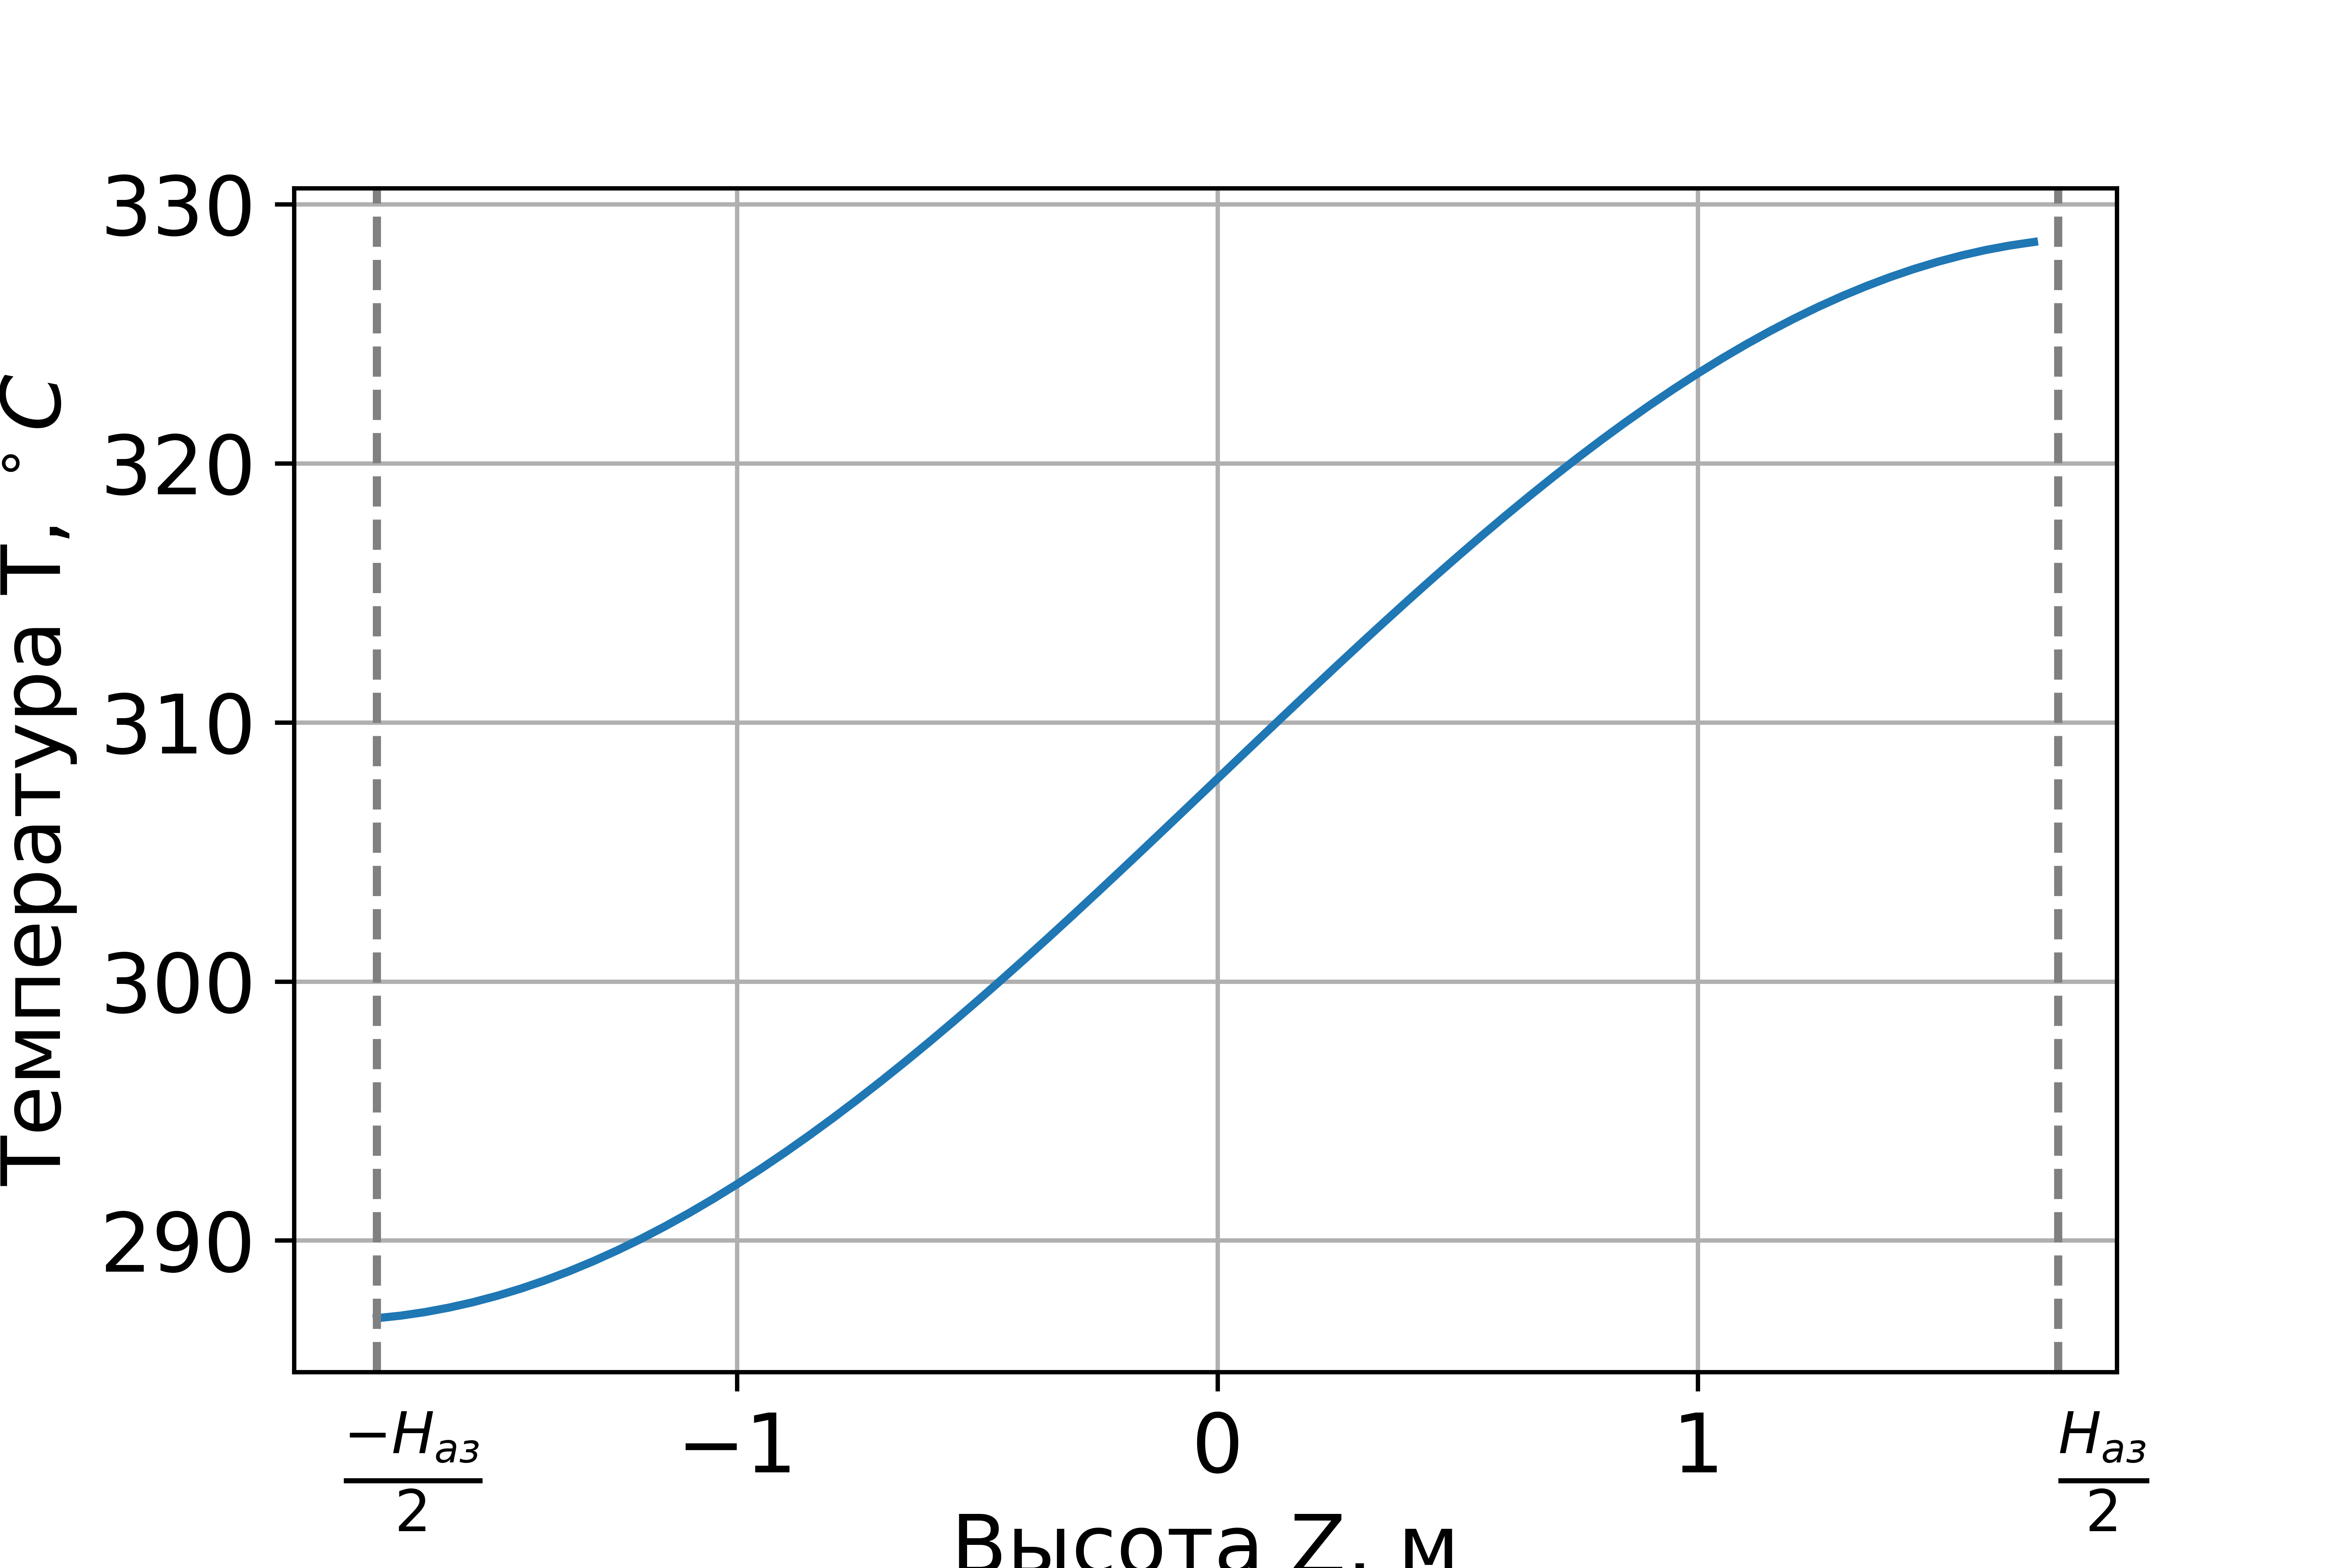
\includegraphics[]{Tz.png}
		\caption{Изменение температуры теплоносителя по высоте}
		\label{pic:TZ} % название для ссылок внутри кода
	\end{center}
\end{figure}

Максимальная температура теплоносителя определяется из температуры кипения теплоносителя при давлении в активной зоне. Температура насыщения воды при давлении $15.7$ МПа — $345.8\  ^\circ C$. Отсюда следует что запас до кипения $\approx 17.26\  ^\circ C$. 

\subsection{Расчет распределения температуры внешней стенки оболочки по высоте}
Площадь проходного сечения:
\begin{equation}
S_{\text{прох}} = \sqrt{3}/2(a - 2 \cdot \delta_{\text{чехла}})^2 - N_{\text{твэл}} \frac {\pi d^2_{\text{тв}}} {4} - N_{\text{н.к.}} \frac {\pi D_{\text{н.к}}^2} {4} - \frac {D_{\text{ц.к}}^2\pi}{4}
\end{equation}
\begin{equation}
S_{\text{прох}} =\sqrt{3}/2(2.340 \cdot 10^{ -01 } - 2 \cdot 0.0015)^2 - 3.170 \cdot 10^{ 2 } \frac { \pi (9.100 \cdot 10^{ -03 })^2 } {4} - 1.200 \cdot 10^{ 1 } \frac { \pi (1.260 \cdot 10^{ -02 }))^2} {4} - \frac { (1.030 \cdot 10^{ -02 })^2\pi } {4} 
\end{equation}
\begin{equation}
S_{\text{прох}} =  2.402 \cdot 10^{ 4 } \text{мм}^2
\end{equation}

Периметр:
\begin{equation}
\Pi= (2(a-2\delta_{\text{чехла}})\sqrt{3}) - N_{\text {твэл }} \pi d_{\text {тв }}+N_{\text {н.к }} \pi D_{\text {н.к }}+\pi D_{\text {ц.к}}
\end{equation}
\begin{equation}
\Pi=(2( \cdot 2.340 \cdot 10^{ -01 }-2 \cdot 1.500 \cdot 10^{ -03 }) \cdot \sqrt{3}) - 3.170 \cdot 10^{ 2 } \cdot \pi \cdot 9.100 \cdot 10^{ -03 } + 1.200 \cdot 10^{ 1 } \cdot \pi \cdot 1.260 \cdot 10^{ -02 } + \pi \cdot 1.030 \cdot 10^{ -02 }
\end{equation}
\begin{equation}
\Pi= 1.037 \cdot 10^{ 4 } \text{мм}
\end{equation}
Гидравлический диаметр:
$$
d_{\text{Г}} = \frac {4 S_{\text{прох}}}{\text{П}}
=
\frac {4 \cdot 2.402 \cdot 10^{ -02 }} {1.037 \cdot 10^{ 1 }} = 9.263 \cdot 10^{ -03 }
 \text{мм}
$$

Определим коэффициент теплоотдачи в режиме турбулентного
стационарного течения несжимаемой жидкости. 
Параметры теплоносителя при усредненной температуре $\overline{T}=303.5 ^\circ \mathrm{C}$:
\begin{itemize}
\item Динамическая вязкость $\mu = 8.721 \cdot 10^{-5} \text{Па} \cdot \text{c}$ 
\item Коэффициент теплопроводности $\lambda = 0.5536 \frac {\text{Вт}}{\text{м} \cdot K}$
\item Число Прандтля $Pr = 0.8729$
\end{itemize}

По формуле Б.С.Петухова, В.В. Кириллова (круглые трубы) \cite{богословская}:

Число Рейнолдса:
$$
\operatorname{Re}=\frac{G_{\text {реак }} \cdot d_{\mathrm{r}}}{N_{\mathrm{TBC}} \cdot S_{\text {npox }} \cdot \mu} = 4.283 \cdot 10^{ 5 }
$$
Коэффициент гидравлического сопротивления:
$$
\xi_{\text{тр}}=(1,82 \cdot \log (\mathrm{Re})-1.64)^{-2}= 1.35 \cdot 10^{-02}
$$
Расчитываем число Нуссельта:
\begin{align*}
\mathrm{Nu}=&\frac{\frac{\xi}{8} \cdot \mathrm{Re} \cdot \operatorname{Pr}}{k+12.7 \cdot\left(\operatorname{Pr}^{\frac{2}{3}}-1\right) \cdot \sqrt{\frac{\xi}{8}}}
=\\=&
\frac{ 
    \frac{1.349 \cdot 10^{ -02 }}{8} \cdot 4.283 \cdot 10^{ 5 } \cdot 8.729 \cdot 10^{ -01 } 
}
{ 
    1 + \frac{900}{4.283 \cdot 10^{ 5 }} + 12.7 \cdot\left((8.729 \cdot 10^{ -01 })^{\frac{2}{3}}-1\right) \cdot \sqrt{\frac{1.349 \cdot 10^{ -02 }}{8}} 
} = 6.589 \cdot 10^{ 2 }
\end{align*}, где $k = 1 + \frac{900}{Re}$  \\
Коэффициент теплоотдачи:
    $$
    \alpha_1 = \frac {Nu \cdot \lambda} {d_\text{г}} = \frac {6.589 \cdot 10^{ 2 } \cdot 5.536 \cdot 10^{ -01 }}{9.263 \cdot 10^{ -03 }} = 3.938 \cdot 10^{ 4 } \frac {\text{Вт}}{\text{м}^2\cdot\mathrm{K}}
    $$
По формуле Диттуса-Болтера \cite{деев}:
    $$
    Nu = 0.023Re^{0.8}Pr^{0.4} = 697.5
    $$
Коэффициент теплоотдачи:
    $$
    \alpha_2 = \frac {Nu \cdot \lambda} {d_\text{г}} = \frac {6.975 \cdot 10^{ 2 } \cdot 5.536 \cdot 10^{ -01 }}{9.263 \cdot 10^{ -03 }} = 4.169 \cdot 10^{ 4 } \frac {\text{Вт}}{\text{м}^2\cdot\mathrm{K}}
    $$
По формула М.А. Михеева \cite{михеев}:
    $$
    Nu = 0.021Re^{0.8}Pr^{0.43} = 634.28
    $$
Коэффициент теплоотдачи:
    $$
    \alpha_3 = \frac {Nu \cdot \lambda} {d_\text{г}} = \frac {6.343 \cdot 10^{ 2 } \cdot 5.536 \cdot 10^{ -01 }}{9.263 \cdot 10^{ -03 }} = 3.791 \cdot 10^{ 4 } \frac {\text{Вт}}{\text{м}^2\cdot\mathrm{K}}
    $$
Усредним коэффициент теплоотдачи:
    $$
    \alpha = \frac {\alpha_1 + \alpha_2 + \alpha_3} {3} = 3.966 \cdot 10^{ 4 } \frac{\text{Вт}}{\text{м}^2 \cdot K}
    $$
Распределение температуры внешней стенки твэла по высоте реактора:
    $$
    T_{\text {об }}(z)=T_{\text {тн }}(z)+\frac{q_{\max } \cdot \cos \left(\frac{\pi \cdot z}{H_{\ni \phi}}\right)}{\pi d_{\text {тв }} \alpha}
    $$
Распределение температуры внешней стенки
твэла по высоте реактора представлено на \ref{pic:Tob}

\begin{figure}[H]
	\begin{center}
		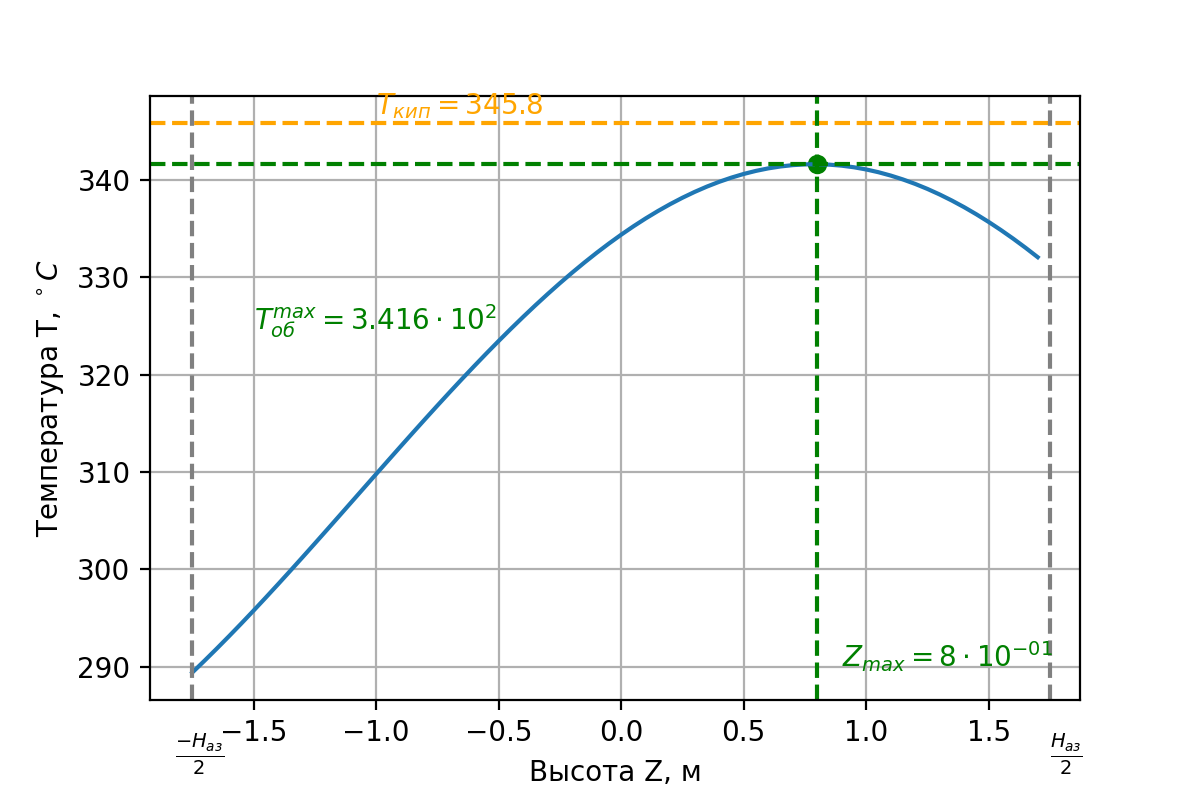
\includegraphics[]{Tob.png}
		\caption{Изменение температуры стенки твэла по высоте}
		\label{pic:Tob} % название для ссылок внутри кода
	\end{center}
\end{figure}

 Из \ref{pic:Tob} 
 видно, что максимальная температура $T_{\text{об}}^{\max} = 341.6 ^\circ C $ стенки достигается в $Z_{\max} = 0.8 м$. Отсюда можно сделать вывод о том, что также отсутствует поверхностное кипения теплоносителя.
 %максимальная температура оболочки в условиях нормальной эксплуатации определяется прочностными и пластическими свойствами сплава и составляет сколь-кот то из справочника

Общий график для распределений теплоносителя и оболочки представлены на \ref{pic:obsh}
\begin{figure}[H]
	\begin{center}
		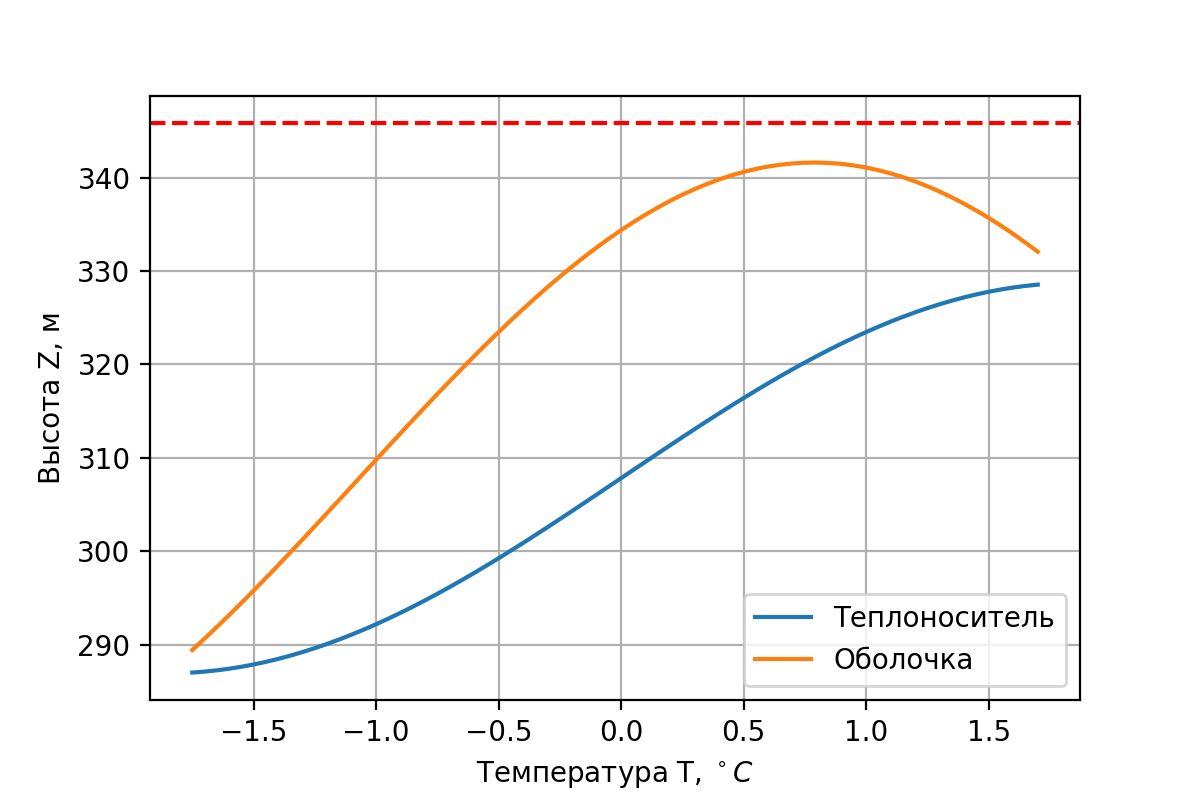
\includegraphics[]{Obsh.png}
		\caption{Изменение температуры стенки твэла и теплоносителя по высоте}
		\label{pic:obsh} % название для ссылок внутри кода
	\end{center}
\end{figure}
    
%NСУЗ — по числу отверстий в канале 

\subsection{Расчет температуры топлива}
    Произведём расчет термического сопротивления оболочки, газового зазора и топлива:
\begin{align*}
\sum R_i =& 
\frac {\ln \frac {d_{\text{тв}}}{d_{\text{тв}} - 2\delta_{об}}  }{2\pi\lambda_{\text{об}}}+\frac {\ln \frac {d_{\text{тв}} - 2\delta_{об}}{d_{\text{топ}}}  }{2\pi\lambda_{\text{г.з}}}+\frac {\frac 1 2 - \frac {d_{\text{отв}}^2} {d_{\text{топ}}^2 - d_{\text{отв}}^2}\ln \frac {d_{\text{топ}}}{d_{\text{отв}}}} {2 \pi \lambda_{\text{топ}}} =
=\\=&
\frac {\ln \frac{ 9.100 \cdot 10^{ -03 } }{ 9.100 \cdot 10^{ -03 } - 2 \cdot 6.500 \cdot 10^{ -04 }} } {2\cdot \pi \cdot 2.010 \cdot 10^{ 1 }}
\\+& \frac {\ln \frac {9.100 \cdot 10^{ -03 } - 2 \cdot 6.500 \cdot 10^{ -04 }}{7.530 \cdot 10^{ -03 }} } {2 \pi \cdot 3.500 \cdot 10^{ -01 }}
\\+& \frac { 0.5 - \frac{ (1.300 \cdot 10^{ -03 })^2 }{ (7.530 \cdot 10^{ -03 })^2 - (1.300 \cdot 10^{ -03 })^2 } \ln \frac { 7.530 \cdot 10^{ -03 } }{ 1.300 \cdot 10^{ -03 } } } {2 \pi \cdot 3.500  }
=\\=&3.752 \cdot 10^{ -02 } \frac {\text{м} \cdot K}{\text{Вт}}
\end{align*}
где
\begin{itemize}
    \item $\lambda_{\text{г.з.}} = 0.35\  \frac {\text{Вт}}{\text{м} \cdot \text{К}}$ — теплопроводность газового слоя 
    \item $\lambda_{\text{об}} = 23\  \frac {\text{Вт}}{\text{м} \cdot \text{К}}$ — теплопроводность оболочки 
    \item $\lambda_{\text{топ}} = 3\  \frac {\text{Вт}}{\text{м} \cdot \text{К}}$ — теплопроводность топлива
\end{itemize}
Распределение температур в топливе по высоте активной зоны:
$$
T_{\text {топ }}(z)=T_{\mathrm{ст}}(z)+\Sigma R_{i} \cdot q_{\max } \cdot \cos \left(\frac{\pi \cdot z}{H_{\text {эф }}}\right)
$$
График изменения температуры топлива по высоте представлен на \ref{pic:top}
\begin{figure}[H]
	\begin{center}
		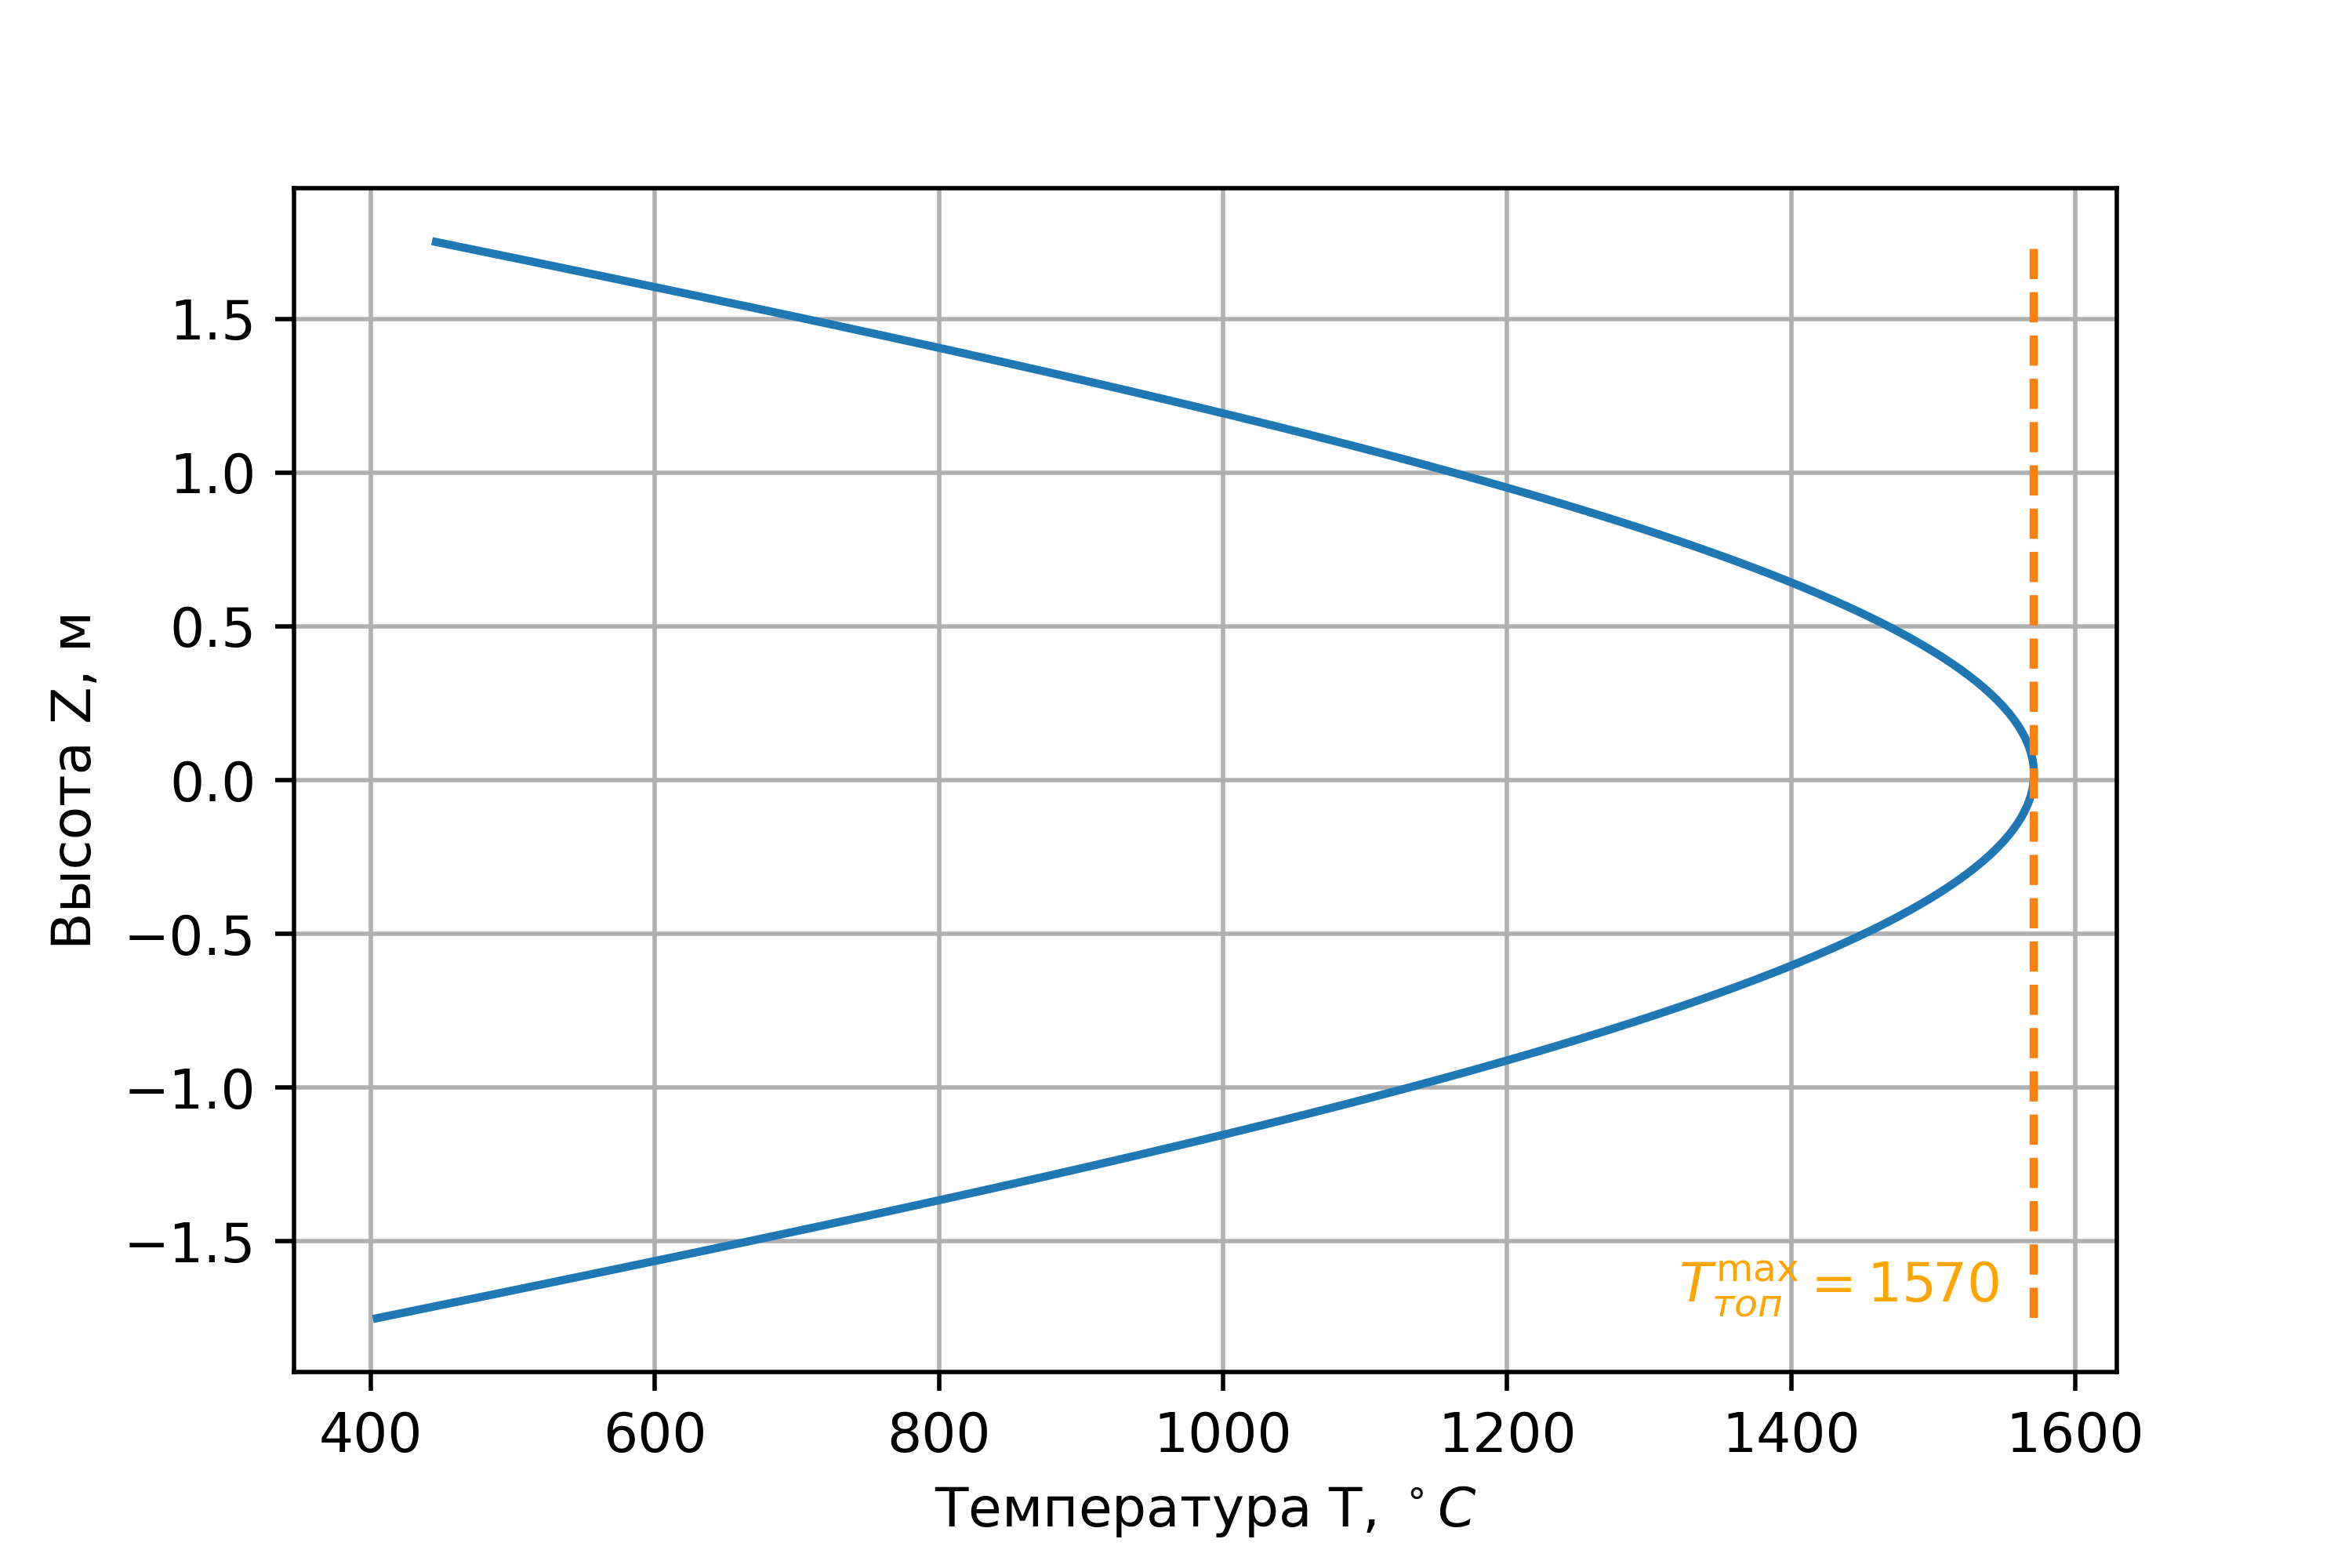
\includegraphics[]{Ttop.png}
		\caption{Изменение температуры топлива по высоте}
		\label{pic:top} % название для ссылок внутри кода
	\end{center}
\end{figure}

Максимальная температура топлива $T_{\text{топ}} = 1559 ^\circ C$ при $Z_{\text{max}} = 0 \text{м}$. Максимально допустимая температура топлива при авариях определяется температурой плавления оксида урана и составляет с некоторым запасом $2600 ^\circ C$. Однако в условиях нормальной эксплуатации максимально допустимая температура топлива определяется сколонностью топлива к усиленному распуханию. % начиная с некоторой температуры, которая равна $1041 ^\circ C$.

\subsection{Определение перепадов давления и необходимой мощности насосов на прокачку}
Для того чтобы определить мощность на прокачку теплоносителя через реактор, найде перепад давления в ТВС
\noindent Гидравлическое сопротивление трения по формуле Дарси:
$$
\Delta P_{\text{тр}}=\xi_{\text{тр}}\cdot\frac{H_{\text{аз}}}{d_{\text{г}}}\cdot \frac {w^2}{2}\rho_{\text{ср}}
=
1.349 \cdot 10^{ -02 } \frac {3.500 } {9.263 \cdot 10^{ -03 }} \cdot \frac {(5.629 )^2} {2} \cdot 7.165 \cdot 10^{ 2 }
=5.785 \cdot 10^{ 4 } \text{Па}
$$
где 
\begin{itemize}
\item $w$, средняя скорость теплоносителя: \begin{equation}w = \frac{G_{\text{реак}}}{\rho_{\text{ср}} \cdot S_{\text{прох}} \cdot N_{\text{ТВС}}}= \frac {1.579 \cdot 10^{ 4 }} {7.165 \cdot 10^{ 2 } \cdot 2.402 \cdot 10^{ -02 } \cdot 1.630 \cdot 10^{ 2 }} = 5.629 \ \text{м} /\text{c}\end{equation}
\item $\rho_{\text{ср}} = 720\ \text{Па}$ — средняя плотность среды
\end{itemize}

\noindent Потеря напора на ускорение:
\begin{equation}
\Delta P_{\mathrm{уск}} = \left( \frac{G_{\text{реак}}}{N_{\mathrm{TBC}} \cdot S_{\mathrm{npox}}} \right)^{2} \cdot \left(\frac{1}{\rho_{\mathrm{вых}}} - \frac{1}{\rho_{\mathrm{вx}}} \right)
=
\left( \frac{ 1.579 \cdot 10^{ 4 } } { 1.630 \cdot 10^{ 2 } \cdot 2.402 \cdot 10^{ -02 } } \right)^2 \cdot \left(\frac 1 { 6.808 \cdot 10^{ 2 } } - \frac 1  { 7.521 \cdot 10^{ 2 } } \right) =  2.265 \cdot 10^{ 3 } \text{Па}
\end{equation}, где $\rho_{\text{вых}} = 680.8\ \frac{\text{кг}}{\text{м}^2} $, $\rho_{\text{вх}} =752.1\  \frac {\text{кг}}{\text{м}^2}$.
\newline
\noindent Нивелирный напор:
$$
\Delta P_{\text{нив}} = \rho_{\text{ср}} \cdot g \cdot H_{\text{аз}}
=
7.165 \cdot 10^{ 2 } \cdot 9.807 \cdot 3.500  = 2.459 \cdot 10^{ 4 } \text{Па}
$$
Местное сопротивление:
$$
\Delta P_{\text{мест}} = \frac{ \left( \frac{1.579 \cdot 10^{ 4 }} {163 \cdot 2.402 \cdot 10^{ -02 } }  \right)^2 } {2} \cdot \left( \frac{ 2.6 }{ 7.521 \cdot 10^{ 2 } } +\frac{ 13 \cdot 0.45 }{7.165 \cdot 10^{ 2 }}+\frac{0.26} { 6.808 \cdot 10^{ 2 } } \right) = 9.761 \cdot 10^{ 4 } \text{Па}
$$
где $\xi_{\text{вх}}= 2.6 $ — коэффициент сопротивления на входе в кассету; $\xi_{\text{вых}} = 0.26$ — коэффициент сопротивления на выходе из кассеты, $\xi_{\text{реш}} = 0.45$ — коэффициент сопротивления при проходе через дистанцирующую решетку %укажи количество дистанцирующих решеток
Общее сопротивление каналов:
$$
\Delta P=\Delta P_{\mathrm{тр}}+\Delta P_{\mathrm{уск}}+\Delta P_{\text { нив }}+\Delta P_{\text {мест }} = 1.823 \cdot 10^{ 5 } \text{Па} 
$$
Мощность, необходимая для прокачки теплоносителя через весь реактор:
$$
N_{\mathrm{пр}}=N_{\mathrm{ТВС}} \frac{\Delta P \cdot G_{\mathrm{TBC}}}{\eta_{\text {нас }} \cdot \rho_{\mathrm{вх}}}
$$, где $\eta_{\text{нас}}=0.8$ — КПД насоса
\[
    N_{\text{пр}} = 163 \cdot \frac {1.823 \cdot 10^{ 5 } \cdot 9.685 \cdot 10^{ 1 }} {0.8 \cdot 7.521 \cdot 10^{ 2 }} = 4.783 \cdot 10^{ 6 } \text{Вт}
\]
\noindent КПД реактора с учетом потерь на прокачку теплоносителя:
$$
\eta^{\prime} = \frac{Q_{\text {эл }}-N_{\text {пр }}}{Q_{\text {теп }}}=\frac{1.000 \cdot 10^{ 9 } - 4.783 \cdot 10^{ 6 }}{2.904 \cdot 10^{ 9 }}={3.427 \cdot 10^{ -01 }}
$$
% \subsection{Определение запаса до кризиса теплообмена}
\subsection{Выводы из теплофизического расчета}
По итогам теплогидравлического расчета были определены основные термодинамические и теплогидравлические параметры РУ ВВЭР-1000. Были выполнены следующие поставленные задачи:
\begin{enumerate}
   \item Произведен выбор турбины и определён её КПД равный 0.342 с учетом мощности, необходимой на прокачку теплоносителя.
   \item Были найдены зависимости температуры оболочки и теплоносителя от высоты АЗ, было выяснено, что поверхностного кипения не наблюдается, и максимальная тепература оболочки твэла 341.6 $^\circ C$ не превышает предельно допустимую.
   \item Определена зависимость температуры топлива от высоты АЗ, максимальная температура топлива $1464 ^\circ C$ не превышает предельное значение $1900 ^\circ C$.
\end{enumerate}

% \section{Нейтронно-физический расчет}
\section{Нейтронно-физический расчет}

\subsection{Постановка задачи}
В рамках данного этапа работы будет выполнены следующие задачи:
\begin{enumerate}
    \item Ячеечный расчет для определения характеристик ТВС в приближении бесконечной решетки
        \subitem Расчет ячеек без выгорания
        \subitem Построение модели полиячеек и их расчет без выгорания
        \subitem Расчет длительности цикла и выгорания при частичных перегрузках
    % \item Расчет энерговыделения и коэффициента неравномерности активной зоны в приближении гомогенизированных ячеек
\end{enumerate}

\subsection{Описание инструмента ячеечного расчета}
Для расчета свойств ТВС использовались возможности программного комплекса GETERA-93 %\cite{белоусов2002использование}. 
Программа представляет собой инструмент для расчета нейтронно-физических характеристик активной зоны методом вероятностей первых столкновений, предоставляющий одномерный расчет активных зон сложной геометрии благодаря полиячеечным расчетам.

Данная программа разрабатывалась для группового расчета полей нейтронов на основе метода вероятностей первых столкновений (ВПС) полей нейтронов в ячейках реакторов, содержащих элементы с различной геометрией.
\subsection{Модель ячейки}
Для проведения расчетов определим исходные характеристики ТВС РУ-ВВЭР-1000 %\cite{ТвэлТерновых} 

\begin{table}[H]
	\caption{Исходные данные для ТВС проектируемого РУ ВВЭР-1000 }
	\begin{center}
        \begin{tabular}{|l|c|}
        \toprule
         Характеристика & Значение \\ 
         \midrule
          Форма ТВС & Шестигранная\\
         \hline
          Количество твэлов в ТВС & 317\\
         \hline
         Топливо & $\text{U}\text{O}_2$ \\
         \hline
         Обогащение топлива, \%& 4.7 \\
         \hline
         Плотность топлива, $\text{г}/\text{см}^3$ & 9.015 \\
         \hline
         Количество циклов перегрузки топлива & 3 \\
         \hline
         Состав оболочки & $99\% \text{Zr} + 1 \% \text{Nb}$ \\
         \hline
         Замедлитель & $\text{H}_2\text{O}$ \\
         \bottomrule
		\end{tabular}
		\label{tabular:neutron_in}
	\end{center}
\end{table}
\subsection{Расчет ячеек без выгорания}
Для расчета использовалась модель одномерной элементарной эквивалентной цилиндрической ячейки c радиусами $0.398, 0.455, 0.67$ мм. Геометрия элементарной ячейки представлена на рисунке \ref{pic:neutron_cell}

\begin{figure}[H]
	\begin{center}
		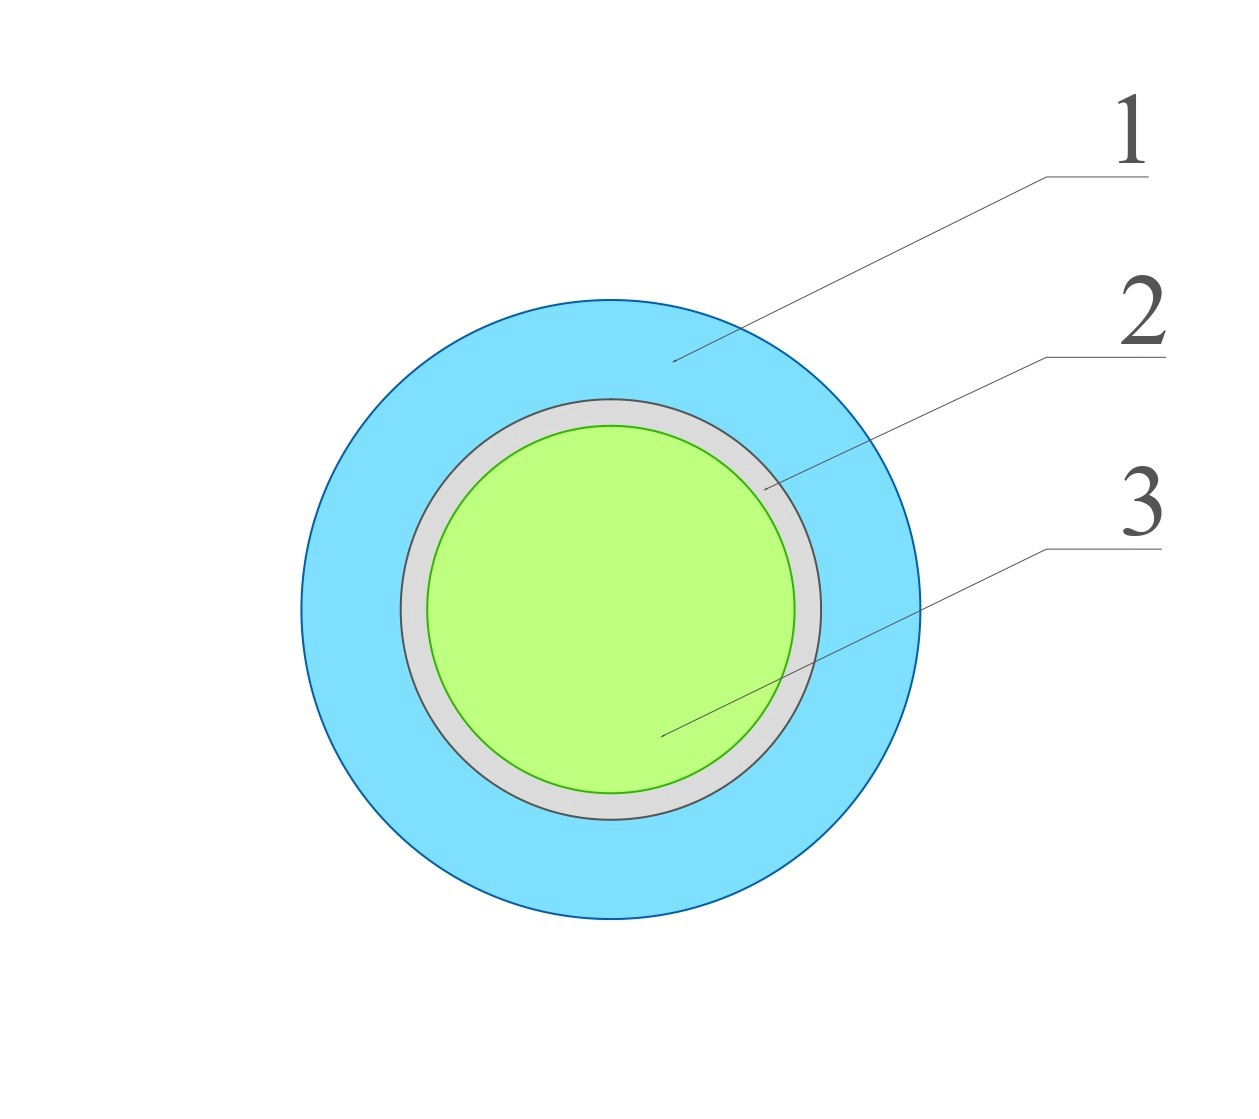
\includegraphics[scale=0.2]{cell.jpg}
		\caption{Геометрия элементарной топливной ячейки. 1 — замедлитель, 2 – оболочка, 3 – топливо}
		\label{pic:neutron_cell} % название для ссылок внутри кода
	\end{center}
\end{figure}
Рассчитаем необходимые концентрации элементов входящих в состав ячейки

\begin{table}[H]
	\caption{Концентрации элементов}
	\begin{center}
        \begin{tabular}{|l|c|}
        \toprule
         Элемент & Концентрация\\ 
         \midrule
          Топливо & \\
         \hline
          $\text{U}^{235}$ & $9.4518 \cdot 10^{-4}$\\
         \hline
          $\text{U}^{238}$ & $1.9165\cdot 10^{-2}$\\
         \hline
          $\text{O}$ & $4.02 \cdot 10^{-2}$\\
         \hline
         Оболочка & \\
         \hline
          $\text{Zr}$ & $4.25047 \cdot 10^{-2}$\\
         \hline
          $\text{Nb}$ & $5.55308\cdot 10^{-4}$\\
         \hline
         Замедлитель & \\
         \hline
         $\text{H}$ & $4.98456\cdot 10^{-2}$\\
         \hline
         $\text{O}$ & $2.49228\cdot 10^{-2}$\\
         \bottomrule
		\end{tabular}
		\label{tabular:neutron_conc}
	\end{center}
\end{table}
Используя входные данные зададим расчетную ячейку с указанными в \ref{tabular:neutron_conc} составами и радиусами.
Произведем расчет $K_{\infty}$ бесконечной решетки твс заданной модели с помощью команды \texttt{:FIER} заданной во входном файле расчета GETERA-93. Результрующее значение:
$$
K_{\infty} = 1.38
$$
\subsection{Расчет полиячеек без выгорания}
Перед дальнейшими расчетами выгорания необходимо усложнить модель активной зоны, представив ее бесконечной решеткой  полиячеек. Такой подход позволит учесть ячейки с различной степенью выгорания в активной зоне для дальнейшего расчета при использовании частичиных перегрузок. 

Разобьём ячейку на 3 фрагмента (в соответствии с заданным количество циклов выгорания), для которых предполагается применимым одномерное приближение. Связи между фрагментами зададим с помощью следующей матрицы перетечек записанной в переменную \texttt{ALOUT} расчетного файла:
$$
\begin{pmatrix}
0.0 & 0.5 & 0.5 \\ 
0.5 & 0.0 & 0.5 \\
0.5 & 0.5 & 0.0
\end{pmatrix}
$$
Повторный расчет заданой поличячейки дает аналогичный результат расчету элементарный ячейки без выгорания, из чего можно сделать вывод что модель полиячейки построена верно.

\subsection{Расчет длительности цикла и выгорания при частичных перегрузках}
Используя полиячеечную модель из предыдущего этапа воспроизведем трехцикловой процесс перегрузок топлива и подберем оптимальное время цикла выгорания при энерговыделении $q_v=110$. Оптимальным будет считать такое время цикла, по прошествии которого $K_{\text{\infty}} = 1.03$, что эквивалентно $K_{\text{eff}} = 1.0$ для нашей модели.

Используя команду \texttt{:CORR} переопределим составы, добавив концентрации свежего топлива во все фрагменты полиячеек последовательно. 

Оптимальное время цикла по резльтатам расчета:
$$
T_{\text{цикла}} = 450\ \text{суток}
$$

В таблице \ref{tabular:burnup} представлены характеристики, полученные из расчета выгорания

\begin{table}[H]
	\caption{{Характеристики процесса выгорания}}
	\begin{center}
        \begin{tabular}{|c|c|}
        \toprule
         Характеристика & Значение\\ 
         \midrule
         \hline
          $K_\infty$ в начале цикла & $1.1667$\\
         \hline
          Длина цикла, сут & 450 \\
         \hline
          Длина кампании, сут & 1350\\
         \hline
          Выгорание, МВт $\cdot$ сут / кг & $53.541$\\
         \hline
          Годовой расход ТВС, 1 / год & 42.2\\
         \hline
          Плутониевый вектор в конце кампании, \% & \\
         \hline
          $\text{Pu}^{38}$ & 1.97 \\
         \hline
          $\text{Pu}^{39}$ & 55.18 \\
         \hline
          $\text{Pu}^{40}$ & 21.35\\
         \hline
          $\text{Pu}^{41}$ & 15.59 \\
         \hline
          $\text{Pu}^{42}$ & 5.91 \\
         \hline
         Содержание делящегося изотопа (Pu39 + Pu41) в \\ отработавшем топливе, кг/тонна топлива & 14.87\\
         \hline
         Содержание делящегося изотопа (U235)\\ в отработавшем топливе, кг/тонна топлива & 11.4 \\
         \hline
         Загрузка делящихся нуклидов, кг/тонна топлива & 47 \\
         \bottomrule
		\end{tabular}
		\label{tabular:burnup}
	\end{center}
\end{table}






% 2 части
% Расчет Характеристик ТВС
% Расчет макро групповых констант для модели активной зоны с гомогенизированными ячейками 
% гомогенизация чтобы применить диффузию

% Плутониевый веткор для изотопного состава
% \section{Расчет биологической защиты} %TODO: убрать для репорта
\subsection{Постановка задачи}
Необходимо рассчитать дозу облучения при стационарном режиме работы ЯЭУ ВВЭР-1000 за биологической защитой

\subsection{Построение расчетной модели биологической защиты}
Для формирования расчетной модели рассмотрим разомкнутую компоновку элементов и помещений ЯЭУ с РУ ВВЭР-1000. Такая компоновка предполагает разделения реакторного и машинного залов в разные здания, что позволяет локализовать возможную аварию и обеспечить большую безопасность.

\begin{figure}[H]
	\begin{center}
		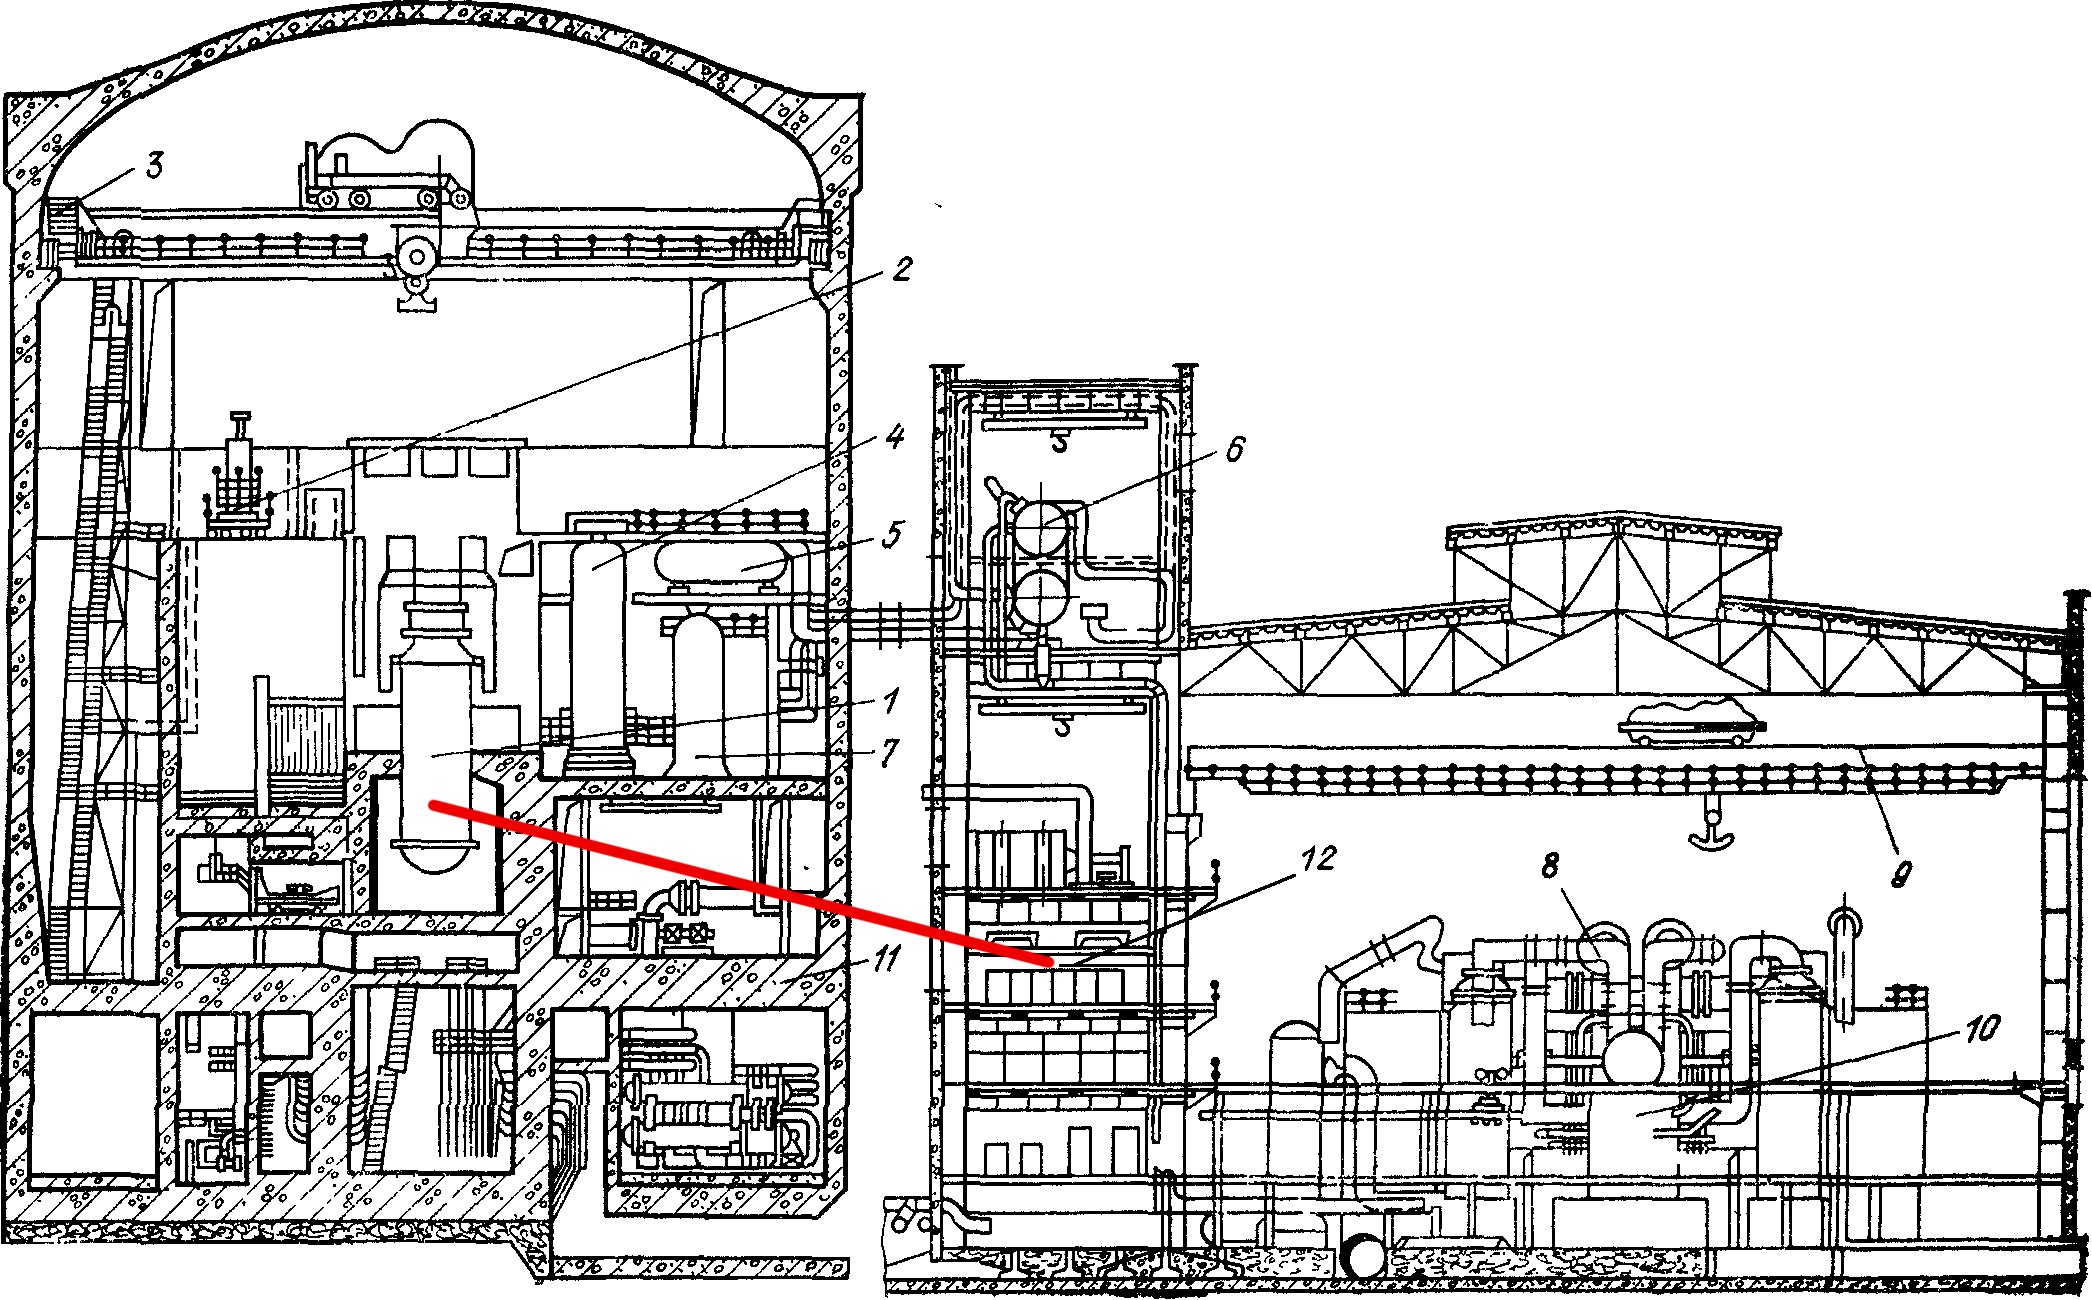
\includegraphics{razrez_bio.png}
		\caption{
			Общая компоновка энергоблока с РУ ВВЭР-1000 разомкнутой компоновки (Южно-Украинская АЭС) \cite{МонаховА.С1986Аэси}: \\
			1 — реактор; 2 — машина для перегрузки топлива; 3 — подъемный кран реакторного отделения; 4 — компенсатор давления, 5 — барботер; 6 — деаэратор; 7 — гидроемкость, 8 — турбогенератор; 9 — подъемный кран машинного зала; 10 — регенеративные подогреватели; 11 — защитная оболочка; 12 — блочный щит управления;
		}
		\label{pic:razrez_bio} % название для ссылок внутри кода
	\end{center}
\end{figure}
% Монахов Атомные электрические станции и их технологическое оборудование

\paragraph{Элементы компоновки вокруг реактора}

Рассмотрим основные элементы защиты, внешние по отношению к ВВЭР-1000 в сборе. Корпус реактора установливается в \textit{бетонную шахту} (рис \ref{pic:beton_shakhta}), которая играет роль основной опоры и крепления реактора с учетом сейсмических нагрузкок, а также биологической защиты от излучения со стороны АЗ. Между корпусом реактора и шахтой имеется кольцевой зазор, предназначенный для периодического контроля металла корпуса в связи с требованиями правил. Шахта резделена по высоте на два объема разделительным сильфоном: 
\begin{itemize}
	\item Верхний, снабжен гидрозатвором и соединяется с бассейном выдержки. При перегрузке верхний объем шахты вместе с бассейном заливается водой.
	\item Нижний, условно разделяемый фермой опорной на шахту зоны патрубков и шахту цилиндрической части корпуса. Соединяется проемом, снабженным герметичной дверью, с помещением для машины осмотра корпуса.
\end{itemize}
В помещении зоны патрубков
биологическая защита выполнена из металлических коробов, заполненных специальным составом, в который входят серпентинитовая галя, кристаллический карбид бора, дробь чугунная литая. В районе активной зоны применяется «сухая» защита, которая представляет из себя слой серпентинитового бетона толщиной
720 мм и высотой 4,7 м, облицованного металлической оболочкой. Такой бетон обладает высокой радиационной стойкостью, что позволяет удовлетворить требования по нейтронной защите. \cite{лескин2011физические}

\begin{figure}[H]
	\begin{center}
		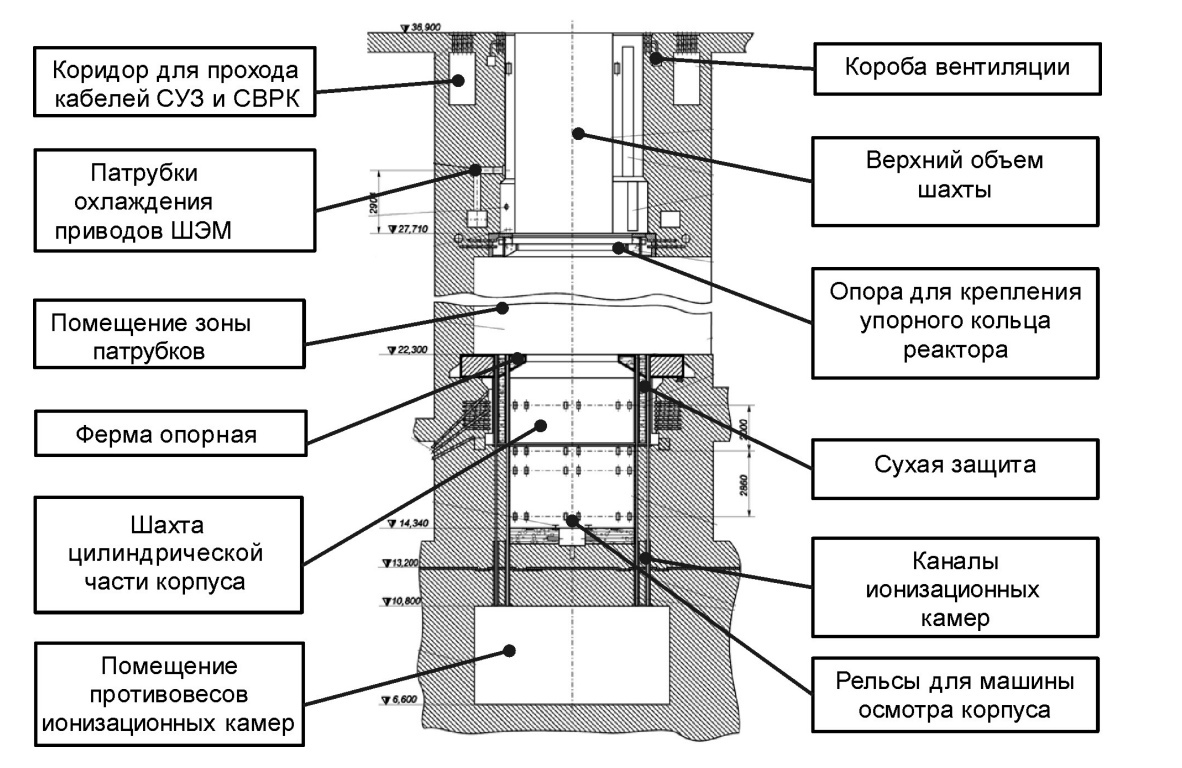
\includegraphics[scale=0.4]{beton.jpg}
		\caption{
			Бетонная шахта реактора 
		}
		\label{pic:beton_shakhta} % название для ссылок внутри кода
	\end{center}
\end{figure}

Все оборудование первого контура заключено в цилиндрическую оболочку, в верхней части которой расположен грузоподъемный поворотный кран. Между реакторным и машинным залами располагается этажерка электротехнических устройств, где размещены также деаэраторы и различные лаборатории.

\paragraph{Корпус и внутрикорпусные элементы компоновки} Корпус представляет собой вертикальный герметичный сосуд
цилиндрической формы с эллиптическими днищем и крышкой  с наружним диаметром 4535 мм, высотой 10.897 м и толщиной 192 мм в цилиндрической части и 210 мм в районе патрубков \cite{лескин2011физические}. В качестве основного материала используется сталь сталь 15Х2НМФА. е. Вся внутренняя поверхность корпуса покрыта
антикоррозионной наплавкой из нержавеющей стали толщиной не
менее 8 мм. В местах соприкосновения корпуса с крышкой, шахтой, уплотнительными прокладками, в местах приварки
кронштейнов, деталей крепления трубок КИП, на поверхности разделительного кольца выполнена наплавка толщиной не менее
15 мм. Внутрь реактора также устанавливается шахта, которая  представляет собой цилиндрическую обечайку с фланцем и эллиптическим днищем, в котором закреплены 163 опорные
трубы (стаканы) с шагом 236 мм, верхние части которых образуют
опорную плиту для установки и дистанционирования кассет активной зоны. Материал шахты – сталь 08Х18Н10Т толщиной 55 мм.

\paragraph{Устройство твэла} Твэл ядерного реактора ВВЭР-1000 представляет собой трубку, заполненную таблетками из двуокиси урана UO2 и герметично уплотненную концевыми деталями на сварке. Трубка твэла изготовлена из циркония, легированного 1 \% ниобия. Наружный диаметр трубки твэла 9.1±0.05 мм, ее толщина 0.65±0.03 мм, а внутренний диаметр 7.72+0.08 мм.
В эту трубку с зазором 0.19–0.32 мм на диаметр помещены таблетки двуокиси урана высотой (длиной) 20 мм и диаметром 7.57±0.04 мм. В середине этих таблеток имеются отверстия диаметром 1.5 мм, а края таблеток скруглены фасками. Общая длина столба этих таблеток в твэле составляет 3530 мм. Все размеры указаны для холодного состояния. Длина трубки твэла составляет 3800 мм, поэтому положение столба топливных таблеток в твэле зафиксировано разрезными втулками из нержавеющей стали и пружиной, не препятствующими тепловым перемещениям. Вид твэла приведён на рис. \ref{pic:tvel} \cite{ТвэлТерновых}

\begin{figure}[H]
    \begin{center}
        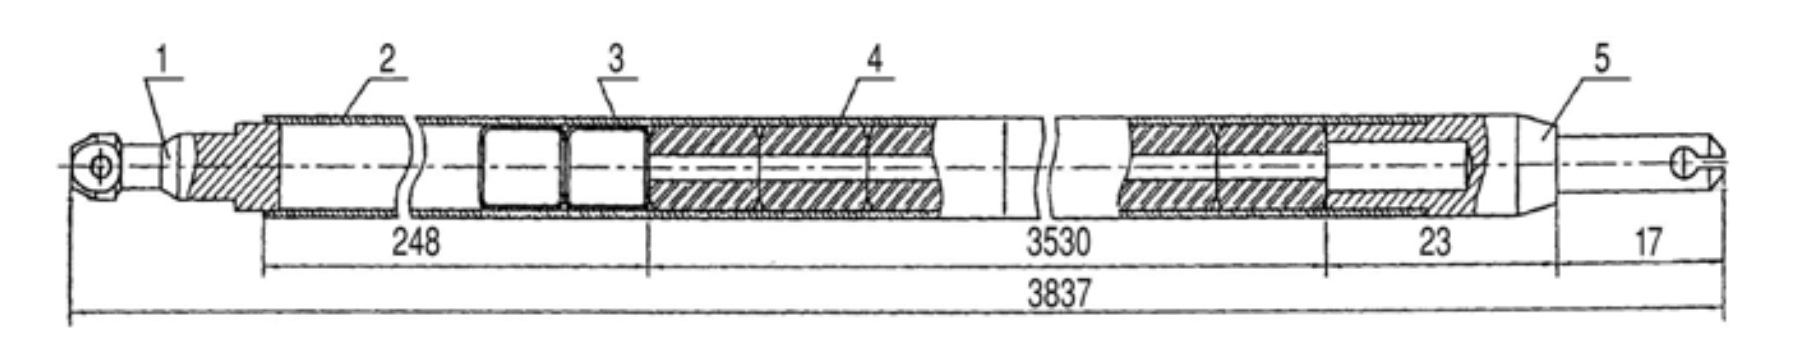
\includegraphics[scale=0.3]{tvel.jpg}
        \caption{
                Тепловыделяющий элемент: 1 – заглушка верхняя; 2 – оболочка; 3 – фиксатор; 4 – таблетка; 5 – заглушка нижняя
        }
        \label{pic:tvel}
    \end{center}
\end{figure}

Преимущество циркония заключается в удачном сочетании ядерных и физических характеристик с механическими и коррозионными свойствами. Цирконий коррозионно стоек в большинстве сред, применяемых в качестве теплоносителей ядерных реакторов, и достаточно технологичен.

Естественная радиоактивность одной свежей ТВС составляет $1.8 \cdot 10^{10}$ Бк., гамма- излучение на поверхности около 0.2 бэр/ч.


\paragraph{Построение одномерной модели} В качестве помещения постоянного пребывания персонала рассматривается блочный щит управления, расположенный в этажерке электроустройств (цифра 12 на рис. \ref{pic:obsh}). Также в этажерке электроустройств размещаются распределительные устройства сетей электропитания двигателей электростанции, аккумуляторные батареи, трансформаторы и т. д.
Для построения расчетной модели был определен ряд значимых элементов конструкции реакторной установки с точки зрения нейтронной защиты. От активной зоны рассматриваемое помещение отделено внутрикорпусными элементами, такими как оболочка твэла, внутрикорпусная шахта; корпусом, бетонной внешней шахтой, внешней бетонной оболочкой реактора и бетонной стеной машинного зала. Суммарный слой бетона складывается из 3 м основания гермооболочки, 0.72 м сухой защиты шахты, 1.5 м шахты и 0.5 м стены машинного зала перед этажеркой.
Основная доля нейтронного излучения в реакторе приходится на нейтроны теплового спектра. Для таких энергий хрошими поглотителями являются кадмий, графит, бетон. 
Присутствующее гамма-излучение для своего эффективного поглощения требует свинец и подобные высокоплотные материалы. Таким образом были выбран слои биологической защиты, представленные в таблице \ref{tabular:bio-sec-layers}:

\begin{table}[H]
	\caption{Слои биологической защиты}
	\begin{center}
        \begin{tabular}{|l|c|c|c|}
        \toprule
         Название & Материал & Размер, см & Плотность, $\text{г}/\text{см}^3$ \\ 
         \midrule
         \hline
         Внутрикорпусная шахта & сталь 08Х18Н10Т & 5.5 & 7.9 \\
         \hline
         Теплоноситель & $\text{H}_2\text{O}$ & 26.3 & 0.71\\
         \hline
         Корпус & сталь 15Х2НМФА & 19.25 & 7.8 \\
         \hline
         Шахта + гермооболочка + стена & бетон & 572 & 2.35 \\
         %\hline
         %Герметичная оболочка & бетон &  & 2.5 \\ 
         \bottomrule
		\end{tabular}
		\label{tabular:bio-sec-layers}
	\end{center}
\end{table}

\subsection{Расчет дозы нейтронов из активной зоны реактора}


\begin{table}[H]
	\caption{Основные параметры для расчета}
	\begin{center}
        \begin{tabular}{|l|c|}
        \toprule
         Параметр & Значение \\ 
         \midrule
         \hline
         Тепловая мощность реактора, МВт $W_{\text{теп}}$ & $2.904 \cdot 10^3$ \\ 
         \hline
         Средняя энергия, выделяющаяся в одной реакции деления, МэВ $E_f$ & 200  \\ 
         \hline
         Средняя энергия нейтронов спектра деления, МэВ $E_{nf}$ & 2 \\
         \hline
         Среднее число нейтронов деления на середину кампани, $\nu_f$ & 2.42 \\
         \hline
         Коэффициент размножения $K_\infty$ & 1.03  \\
         \hline
         Доля нейтронов спектра деления в спектре утечки $\gamma$ & 0.5 \\
         \hline
         Среднее число гамма-квантов деления на середину кампании & 7.51 \\
         \hline
         Высота активной зоны $H_{\text{аз}}$, м & 3.5 \\
         \hline
         Радиус активной зоны $R_{\text{аз}}$, м & 1.58 \\
         \bottomrule
		\end{tabular}
		\label{tabular:bio_sec_in}
	\end{center}
\end{table}


\noindent Число реакций деления в реакторе в единицу времени:
\begin{equation}
        N_f = \frac
               { W_{ \text{теп} } }
        %   -------------------------
                   { E_f  }
\end{equation}
$$
       N_f = \frac
                     { 2.90 \cdot 10^{{ 9 }} }
 %   -------------------------------------------------------
    { 2.00 \cdot 10^{{ 2 }} \cdot 1.60 \cdot 10^{{ -13 }} }
= 9.06 \cdot 10^{{ 19 }}
\ \frac{\text{дел} } {\text{с} }
$$

\noindent Число нейтронов, образующихся в реакторе в единцу времени:
\begin{equation}
        N_n = N_f \cdot \nu_f
\end{equation}
$$
        N_n = 9.06 \cdot 10^{{ 19 }} \cdot 2.42  = 2.19 \cdot 10^{{ 20 }} \ \frac{нейтронов} {с}
$$

\noindent Площадь полной поверхности акивной зоны
\begin{equation}
        S_{\text{пов}} = S_{\text{бок}} + 2S_{\text{top}}
\end{equation}
\noindent где
\begin{itemize}
        \item $S_\text{бок} = H_{\text{аз}}2 \pi R_{\text{аз}}$
        \item $S_{\text{top}} = \pi R_{\text{аз}} ^ 2$
\end{itemize}
$$
        S_{\text{пов}} = 3.50  \cdot 2 \cdot \pi \cdot 1.58  + 2 \cdot \pi \cdot (1.58 )^2 = 5.04 \cdot 10^{{ 1 }}\ \text{м}^2
$$

\noindent Поток нейтронов утечки из активной зоны:
\begin{equation}
        \Phi = \frac
                   {N_n(K_\infty - 1)}
              % ------------------------
                   {S_{\text{пов}}}
\end{equation}
$$
        \Phi = \frac{2.19 \cdot 10^{{ 20 }} (1.03  - 1)} {5.04 \cdot 10^{{ 1 }}} = 1.30 \cdot 10^{{ 17 }}\ \frac{\text{нейтрон}}{\text{с} \cdot \text{м}^2}
$$

\noindent Поток нейтронов спектра деления в утечке из активной зоны:
\begin{equation}
        \Phi_f = \Phi \cdot \gamma
\end{equation}
$$
        \Phi_f = 1.30 \cdot 10^{{ 17 }} \cdot 5.00 \cdot 10^{{ -01 }} = 6.52 \cdot 10^{{ 16 }}\ \frac{\text{нейтрон}} {\text{с} \cdot \text{м}^2}
$$

\noindent Мощность экивалентной дозы нейтронов перед защитой
\begin{equation}
        D_{0n} = \Phi_f \cdot E_{nf} \cdot \overline{\mu_{\text{ЭН}}} \cdot K 
\end{equation}
\noindent где
\begin{itemize}
        \item $\overline{\mu_{\text{ЭН}}} = \frac {1\ \text{м}^2} {100\ \text{кг}}$ — массовый коэффициент поглощения энергии в биологической ткани, принимается равным отношению площади человека к его массе
        \item $K = 10\ \frac {\text{Зв}}{\text{Гр}}$ — коэффициент качества нейтронов спектра деления
\end{itemize}
$$
        D_{0n} = 6.52 \cdot 10^{{ 16 }} \cdot 2.00  \cdot 1.60 \cdot 10^{{ -13 }} \cdot 1.00 \cdot 10^{{ -02 }} \cdot 1.00 \cdot 10^{{ 1 }} = 2.09 \cdot 10^{{ 3 }}\ \frac{\text{Зв}}{\text{c}}
$$
Результаты расчетов дозы нейтронов из активной зоны представлены в таблице \ref{tabular:bio_sec_1_out}

\begin{table}[H]
	\caption{Результаты расчета дозы нейтронов}
	\begin{center}
        \begin{tabular}{|l|c|}
        \toprule
         Параметр & Значение \\
         \midrule
         \hline
         $N_f$, $\frac{\text{дел}}{\text{с}}$ & $9.06 \cdot 10^{19}$ \\ 
         \hline
         $N_n$, $\frac{\text{нейтрон}}{\text{с}}$ & $2.19 \cdot 10^{20}$ \\
         \hline
         $S_{\text{пов}}$, $\text{м}^2$ & $50.4$ \\
         \hline
         $\Phi, \frac{\text{нейтрон}}{\text{м}^2 \cdot \text{с}}$ & $1.3 \cdot 10^{17}$\\
         \hline
         $\Phi_f, \frac{\text{нейтрон}}{\text{м}^2 \cdot \text{с}}$ & $6.52 \cdot 10^{16}$ \\
         \hline
         $D_{0n}, \frac{\text{Зв}}{\text{с}}$ & $2.09 \cdot 10^3$ \\
         \bottomrule
		\end{tabular}
		\label{tabular:bio_sec_1_out}
	\end{center}
\end{table}


\subsection{Расчет дозы нейтронов за защитой или минимального размера слоя биологической защиты для нейтронов}
Для расчета дозы нейтронов за защитой используется модель сечения выведения многослойной системы.

\noindent Сечение выведение для многослойной системы:

\begin{equation}
        D = D_0 \exp\left(
                - \sum_i \Sigma_{\text{rem}}^i \cdot d_i
        \right)
\end{equation}

\noindent Для текущей модели раскрывается как:

\begin{equation}
        D = D_0 \exp\left(
                - \Sigma_{\text{rem}}^{\text{H}_2\text{O}} \cdot d_{\text{H}_2\text{O}}
                - \Sigma_{\text{rem}}^{\text{ст}} \cdot d_{\text{ст}}
                - \Sigma_{\text{rem}}^{\text{ж/б}} \cdot d_{\text{ж/б}}
        \right)
\end{equation}
\noindent где $\Sigma_{\text{rem}}^{\text{H}_2\text{O}}$ — сечение выведеня слоя воды,
              $\Sigma_{\text{rem}}^{\text{ст}}$ — сечение выведения слоя стали,
              $\Sigma_{\text{rem}}^{\text{ж/б}}$ — сечение выведения слоя бетона,
              $d_{\text{H}_2\text{O}}, d_{\text{ст}}, d_{\text{ж/б}}$ — толщины слоев воды, стали и бетона


\begin{table}[H]
	\caption{Значения сечений выведений защиты и толщины различных слоев \cite{ТвэлТерновых}}
	\begin{center}
        \begin{tabular}{|l|c|c|c|}
        \toprule
         Слой защиты & d, см & $\rho, \frac{\text{г}}{\text{см}^3}$ & $\Sigma_{\text{rem}}$, $\text{см}^{-1}$\ \\
         \midrule
         \hline
         Вода & 26.3 & 0.71 & 0.069 \\
         \hline
         Сталь & 24.75 & 7.9 & 0.166 \\
         \hline
         Бетон & 572 & 2.35 & 0.08 \\
         \bottomrule
		\end{tabular}
		\label{tabular:bio_sec_2_in}
	\end{center}
\end{table}
% TODO: все формулы в equation, числовые выражения -- в далары
$$
        D_n = 2.09 \cdot 10^{{ 3 }} \exp\left( 
                -6.90 \cdot 10^{{ -02 }}\cdot2.63 \cdot 10^{{ 1 }}
                -1.66 \cdot 10^{{ -01 }}\cdot2.48 \cdot 10^{{ 1 }}
                -8.00 \cdot 10^{{ -02 }}\cdot5.72 \cdot 10^{{ 2 }}
        \right) = 7.49 \cdot 10^{{ -20 }}\ \frac{\text{Зв}}{\text{с}}
$$
\noindent Для учета 20\% погрешности по дозе модели сечения выведения необходимо использовать поправочный коэффициент 1.2. Итоговая доза с учетом погрешности в Зв / нед:
$$
        D_{n, \text{нед}} = 1.2 \cdot 7 \cdot 24 \cdot 60 \cdot 60 \cdot 7.490 \cdot 10^{{ -20 }} = 5.436 \cdot 10^{{ -14 }}\ \frac{\text{Зв}}{\text{нед}}
$$


\subsection{Расчет дозы гамма-квантов из активной зоны}
Для расчета гамма-квантов перед защитой применен приближенный алгоритм. Его идея – оценить поток гамма-квантов деления из активной зоны реактора в одномерной геометрии и внести поправку на утечку гамма-квантов от других их источников.

\noindent Число гамма-квантов, образующихся в реакторе в единицу времени: 
\begin{equation}
        I = N_f \cdot \nu_\gamma \cdot N_\gamma
\end{equation}
\noindent где $N\gamma$ — доля гамма-квантов определенной энергии в реакции деления, для
E=3 МэВ $N_{\gamma, 3 \text{МэВ}}=0.2$, для E=5 МэВ $N_{\gamma, 5 \text{МэВ}} = 0.15$
Тогда число гамма-квантов в единицу времени для двух энергий:
\begin{align*}
        I_{3\ \text{МэВ}} &= 9.064 \cdot 10^{{ 19 }} \cdot 2.000 \cdot 10^{{ -01 }} \cdot 7.510  = 1.361 \cdot 10^{{ 20 }}\ \frac{\text{кв}}{\text{с}} \\
        I_{5\ \text{МэВ}} &= 9.064 \cdot 10^{{ 19 }} \cdot 1.500 \cdot 10^{{ -01 }} \cdot 7.510  = 1.021 \cdot 10^{{ 20 }}\ \frac{\text{кв}}{\text{с}}
\end{align*}
Рассмотрим перенос нерассеянных гамма-квантов в однородной пластине с внешним источником, перпендикулярным границам пластины. При этом потребуем выполнения следующих условий:
\begin{enumerate}
        \item  толщина пластины равна $L$ – средней ходе активной зоны $L = \frac{4 V_{\text{аз}}}{S_{\text{пов}}}$, где $V_{\text{аз}}$ – объем активной зоны
        \item линейный коэффициент ослабления пластины $\mu_\gamma$ вычисляется через коэффициенты ослабления элементарной ячейки реактора
        \begin{equation}
                \mu_\gamma = \mu_U\varepsilon_U + \mu_{\text{об}}\varepsilon_{\text{об}}+\mu_{\text{т/н}}\varepsilon_{\text{т/н}} + \mu_{\text{зам}}\varepsilon_{\text{зам}}
        \end{equation}
        где $\varepsilon_i$ – объемные доли топлива, конструкционных материалов, теплоносителя и замедлителя в элементарной ячейке.
\end{enumerate}

\begin{table}[H]
	\caption{Объемные доли материалов}
	\begin{center}
        \begin{tabular}{|l|c|}
        \toprule
         Материал & Обьемная доля $\varepsilon_i$ \\
         \midrule
         \hline
         Топливо & 0.166 \\
         \hline
         Оболочка (Zr) & 0.071 \\
         \hline
         теплоноситель/замедлитель (вода) & 0.733 \\
         \bottomrule
		\end{tabular}
		\label{tabular:objem_doli}
	\end{center}
\end{table}

\begin{table}[H]
	\caption{Линейные коэффициенты ослабления $\mu$ для гамма-квантов с энергией 3 и 5 МэВ}
	\begin{center}
        \begin{tabular}{|l|c|c|}
        \toprule
         Материал & $\mu_3, \text{см}^{-1}$ & $\mu_5, \text{см}^{-1}$ \\
         \midrule
         \hline
         Топливо & 0.81 & 0.83 \\
         \hline
         Оболочка (Zr) & 0.237 & 0.221\\
         \hline
         теплоноситель/замедлитель (вода) & 0.028 & 0.021\\
         \bottomrule
		\end{tabular}
		\label{tabular:koeff_oslab}
	\end{center}
\end{table}
\noindent Таким образом полный линейный коэффициент ослабления для энергий E=3 МэВ, 5 Мэв:
\begin{align*}
        \mu_{\gamma, 3\ \text{Мэв}} &= 1.66 \cdot 10^{{ -1 }}\cdot8.10 \cdot 10^{{ -1 }} + 7.10 \cdot 10^{{ -2 }}\cdot2.37 \cdot 10^{{ -1 }} + 7.33 \cdot 10^{{ -1 }}\cdot2.80 \cdot 10^{{ -2 }}\\ &= 1.72 \cdot 10^{{ -1 }}\ \text{см}^{-1} \\
\\
    \mu_{\gamma, 5\ \text{Мэв}} &= 1.66 \cdot 10^{{ -1 }}\cdot8.30 \cdot 10^{{ -1 }} + 7.10 \cdot 10^{{ -2 }}\cdot2.21 \cdot 10^{{ -1 }} + 7.33 \cdot 10^{{ -1 }}\cdot2.10 \cdot 10^{{ -2 }} \\&= 1.69 \cdot 10^{{ -1 }}\ \text{см}^{-1}
\end{align*}
\noindent Объем активной зоны:
$$
V_{\text{аз}} = \pi R_{\text{аз}}^2 H_{\text{аз}} = \pi \cdot 1.58 ^ 2 \cdot 3.5 ^ 2 = 27.45 \text{м}^3
$$

\noindent Толщина пластины:
$$
L = \frac{4 \cdot 27.45} {5.04 \cdot 10^1} = 2.18 \text{м} = 217.7 \text{см}
$$
\noindent Источник гамма-квантов, равномерно распределенный по объему пластины:
\begin{equation}
        Q = \frac I L
\end{equation}
\begin{align*}
        Q_{3\ \text{Мэв}} = \frac{1.361 \cdot 10^{{ 20 }}}{2.177 \cdot 10^{{ 2 }}} = 6.253 \cdot 10^{{ 17 }} \frac{\text{кв}}{\text{с} \cdot \text{см}} \\
        Q_{5\ \text{Мэв}} = \frac{1.021 \cdot 10^{{ 20 }}}{2.177 \cdot 10^{{ 2 }}} = 4.690 \cdot 10^{{ 17 }} \frac{\text{кв}}{\text{с} \cdot \text{см}} \\
\end{align*}
\noindent Число нерассеянных гамма-квантов через поверхность пластины
\begin{equation}
        N = \frac{Q}{\mu_\gamma}\left(1 - \exp\left(-\mu_\gamma L\right)\right)
\end{equation}
\begin{align*}
        N_{3\ \text{МэВ}} = \frac{6.25 \cdot 10^{{ 17 }}}{1.72 \cdot 10^{{ -1 }}} \cdot \left( 1 - \exp\left(-1.72 \cdot 10^{{ -1 }}\cdot2.18 \cdot 10^{{ 2 }}\right)\right) = 3.64 \cdot 10^{{ 18 }} \frac{\text{кв}}{\text{с}} \\
        N_{5\ \text{МэВ}} = \frac{4.69 \cdot 10^{{ 17 }}}{1.69 \cdot 10^{{ -1 }}} \cdot \left( 1 - \exp\left(-1.69 \cdot 10^{{ -1 }}\cdot2.18 \cdot 10^{{ 2 }}\right)\right) = 2.78 \cdot 10^{{ 18 }} \frac{\text{кв}}{\text{с}}
\end{align*}
\noindent Поток нерассеянных гамма-квантов деления из активной зоны:
\begin{equation}
        \Phi_\gamma = \frac N {S_{\text{пов}}}
\end{equation}
\begin{align*}
        \Phi_{\gamma, 3\ \text{МэВ}} = \frac{3.64 \cdot 10^{{ 18 }}}{5.04 \cdot 10^{{ 5 }}}  = 7.22 \cdot 10^{{ 12 }} \frac{\text{кв}}{\text{см}^2 \cdot \text{с}} \\
        \Phi_{\gamma, 5\ \text{МэВ}} = \frac{2.78 \cdot 10^{{ 18 }}}{5.04 \cdot 10^{{ 5 }}}  = 5.51 \cdot 10^{{ 12 }} \frac{\text{кв}}{\text{см}^2 \cdot \text{с}} 
\end{align*}

\noindent Полный поток гама-квантов из активной зоны с учетом поправочного коэффициента $\xi=2$:
\begin{equation}
        \Phi_\gamma^{\text{full}} = \Phi_\gamma \xi
\end{equation}
\begin{align*}
        \Phi_{\gamma, 3\ \text{МэВ}}^{\text{full}} = 7.22 \cdot 10^{{ 12 }} \cdot 2  = 1.44 \cdot 10^{{ 13 }} \frac{\text{кв}}{\text{см}^2 \cdot \text{с}} \\
    \Phi_{\gamma, 5\ \text{МэВ}}^{\text{full}} = 5.51 \cdot 10^{{ 12 }} \cdot 2  = 1.10 \cdot 10^{{ 13 }} \frac{\text{кв}}{\text{см}^2 \cdot \text{с}} 
\end{align*}

\noindent Мощность эквивалентной дозы гамма-квантов перед защитой
\begin{equation}
        D_{0\gamma}=\Phi_\gamma^{\text{full}} \cdot E \cdot \overline{\mu_{\text{ЭН}}} \cdot K
\end{equation}
\begin{align*}
        D_{0\gamma, 3\ \text{МэВ}} = 1.44 \cdot 10^{{ 13 }} \cdot 3 \cdot 1.60 \cdot 10^{{ -13 }} \cdot 100 \cdot 1 = 6.94 \cdot 10^{{ 2 }}\ \frac{\text{Зв}}{\text{c}} \\
        D_{0\gamma, 5\ \text{МэВ}} = 1.10 \cdot 10^{{ 13 }} \cdot 5 \cdot 1.60 \cdot 10^{{ -13 }} \cdot 100 \cdot 1 = 8.82 \cdot 10^{{ 2 }}\ \frac{\text{Зв}}{\text{c}}
\end{align*}
Результат расчета дозы гамма квантов из активной зоны для энергий 3, 5 МэВ представлены в таблицах \ref{tabular:bio_sec_3_out_3}, \ref{tabular:bio_sec_3_out_5} соответственно.

\begin{table}[H]
	\caption{Результаты расчета дозы гамма-квантов энергии 3 МэВ}
	\begin{center}
        \begin{tabular}{|l|c|}
        \toprule
         Параметр & Значение \\
         \midrule
         \hline
         $I_3, \text{кв}{с}$ & $1.36 \cdot 10^{20}$ \\
         \hline
         $L$, см & 217.7 \\
         \hline
         $Q_3$, кв / (см $\cdot$ c)  & $6.25 \cdot 10^{17}$ \\
         \hline
         $\Phi_\gamma 3$, $\frac{\text{кв}}{\text{см}^2 \cdot \text{с}}$ & $7.22 \cdot 10^{12}$ \\
         \hline
         $N_3$, кв / c & $3.64 \cdot 10^{18}$ \\ 
         \hline
         $D_{0\gamma\ 3}$, Зв / c & 694\\
         \hline
         \bottomrule
		\end{tabular}
		\label{tabular:bio_sec_3_out_3}
	\end{center}
\end{table}

\begin{table}[H]
	\caption{Результаты расчета дозы гамма-квантов энергии 5 МэВ}
	\begin{center}
        \begin{tabular}{|l|c|}
        \toprule
         Параметр & Значение \\
         \midrule
         \hline
         $I_5, \text{кв}{с}$ & $1.02 \cdot 10^{20}$ \\
         \hline
         $L$, см & 217.7 \\
         \hline
         $Q_5$, кв / (см $\cdot$ c)  & $4.69 \cdot 10^{17}$ \\
         \hline
         $\Phi_\gamma 5$, $\frac{\text{кв}}{\text{см}^2 \cdot \text{с}}$ & $5.51 \cdot 10^{12}$ \\ 
         \hline
         $N_5$, кв / c & $2.78 \cdot 10^{18}$ \\ 
         \hline
         $D_{0\gamma\ 5}$, Зв / c & 882\\
         \hline
         \bottomrule
		\end{tabular}
		\label{tabular:bio_sec_3_out_5}
	\end{center}
\end{table}
\subsection{Расчет дозы гамма-квантов за защитой или минимального размера слоя биологической защиты для гамма-квантов}
Для расчета дозы гамма-квантов за защитой или минимального размера слоя биологической защиты для гамма-квантов примиенена модель дозовых факторов накоплений.
Эквивалентная дозы нерассеянных гамма-квантов:
\begin{equation}
        D_\gamma = D_{0\gamma}\exp\left(
                -\sum_i\mu_{\gamma i} d_i
        \right)
\end{equation}
\noindent где $\mu_{\gamma i}$ — линейный коэффициент ослабления i-го слоя, $d_i$ — толщина i-го слоя
\begin{table}[H]
	\caption{Линейные коэффициенты ослабления $\mu$ для гамма-квантов с энергией 3 и 5 МэВ за активной зоной}
	\begin{center}
        \begin{tabular}{|l|c|c|}
        \toprule
         Материал & $\mu_3, \text{см}^{-1}$ & $\mu_5, \text{см}^{-1}$ \\
         \midrule
         \hline
         Сталь & 0.3 & 0.25 \\
         \hline
         Бетон & 0.08 & 0.07\\
         \hline
         Вода & 0.028 & 0.021\\
         \bottomrule
		\end{tabular}
		\label{tabular:koeff_oslab_2}
	\end{center}
\end{table}
\begin{align*}
        D_{\gamma, \text{нерас}, 3\ \text{МэВ}} &= 6.94 \cdot 10^{{ 2 }} \cdot \exp (
                - 3.00 \cdot 10^{{ -1 }} \cdot 2.48 \cdot 10^{{ 1 }}
                - 8.00 \cdot 10^{{ -2 }} \cdot 5.72 \cdot 10^{{ 2 }}
                \\ &- 2.80 \cdot 10^{{ -2 }} \cdot 2.63 \cdot 10^{{ 1 }}
        ) = 2.65 \cdot 10^{{ -21 }}\ \frac{\text{Зв} }{\text{с}} \\
        D_{\gamma, \text{нерас}, 5\ \text{МэВ}} &= 8.82 \cdot 10^{{ 2 }} \cdot \exp (
                - 2.50 \cdot 10^{{ -1 }} \cdot 2.48 \cdot 10^{{ 1 }}
                - 7.00 \cdot 10^{{ -2 }} \cdot 5.72 \cdot 10^{{ 2 }}
                \\ &- 2.10 \cdot 10^{{ -2 }} \cdot 2.63 \cdot 10^{{ 1 }}
        ) = 4.26 \cdot 10^{{ -18 }}\ \frac{\text{Зв} }{\text{с} }        
\end{align*}
Дозовый фактор, равный отношению эквивалентной дозы гамма-излучения для квантов всех энергий к эквивалентной дозе излучения нерасеянных гамма-квантов от одного источника
\begin{equation}
        B_D = \frac{D_{\text{нерас}} - D_{\text{рас}}}{D_{\text{нерас}}} = 1 + \frac{D_{\text{рас}}}{D_{\text{нерас}}}
\end{equation}
Тогда полная доза гамма-квантов за защитой:
\begin{equation}
        D_{\text{полн}} = B_D\cdot D_{\text{нерас}}
\end{equation}
Для нахождения фактора накоплени гомогенной среды можно применить формулу Тейлора:
\begin{equation}
        B(\mu d) = A_1\exp(-\alpha_1 \mu d) + (1 - A_1)\exp(- \alpha_2 \mu d)
\end{equation}
По формуле Д.Л. Бродлера:
\begin{equation}
        B_{ \text{гет} } =
        B_N \left( \sum_i^N \mu_i d_i \right)
        + \sum_{ n = 1 }^{ N - 1 } \left[
                B_n \left( \sum_i^n \mu_i d_i \right) 
                - B_{ n + 1 } \left( \sum_i^n \mu_i d_i3\right)
        \right]
\end{equation}
\noindent где $B_j \left( \sum_i^n\mu_i d_i \right)$ — фактор накопения, вычисляемые по формуле Тейлора. Тогда:
\begin{align*}
        B_{\text{гет}\ 3\ \text{МэВ}} &= 92.3 \\
        B_{\text{гет}\ 5\ \text{МэВ}} &= 34.7 \\
\end{align*}
\noindent Полная доза гамма-квантов за защитой:
\begin{align*}
        D_{\gamma\ 3\ \text{МэВ}} = 92.3 \cdot 2.65 \cdot 10^{ - 21}= 2.45 \cdot 10^{-19}\ \frac{\text{Зв}}{\text{с}}\\
        D_{\gamma\ 5\ \text{МэВ}} = 34.7 \cdot 4.26 \cdot 10^{ - 18}= 1.48 \cdot 10^{- 16 }\ \frac{\text{Зв}}{\text{с}}\\
\end{align*}
Мощность эквивалентной дозы, создаваемой гамма-квантами всех энергий за защитой в Зв / нед:
$$
D_\gamma = 7 \cdot 24 \cdot 60 \cdot 60 \cdot (D_{\gamma\ 3\ \text{МэВ}} + D_{\gamma\ 5\ \text{МэВ}}) = 8.95 \cdot 10^{ - 11 } \frac{\text{Зв}}{\text{нед}}
$$

Суммарная мощность, создаваемая за защитой нейтронами и гамма-квантами c учетом погрешности метода фактора накопления:
$$
D = 1.15(D_n + D_\gamma) = 1.15 \cdot (5.44 \cdot 10^{-14} + 8.95 \cdot 10^{-11}) = 1.03 
\cdot 10^{- 10}\ \text{Зв} / \text{нед}
$$

\subsection{Выводы из расчета биологической защиты}
В работе проводился расчет биологической защиты, была проведена оценка мощностей эквивалентных доз нейтронов и гамма-квантов за защитой.

Оценка проводилась для нейтронных потоков методом сечения выведения для системы со слоями, а также для гамма-квантов с энергиями 3 и 5 МэВ методом дозовых факторов накопления.

По результату работы было получена суммарная мощность эквивалентной дозы нейтронов и гамма-квантов за защитой не превышает $1.03 \cdot 10^{- 7} \frac{\text{мЗв}}{\text{нед}}$. Получившаяся доза сильно меньше предельной поглощенной дозы для персонала АЭС, которая составляет $0.4 \frac{\text{мЗв}}{\text{нед}}$, из чего можно сделать вывод, что рассматриваемое помещение БЩУ безопасно с точки зрения радиационной защиты


\section{Исследование полей энерговыделения и теплогидравлических параметров при разных режимах работы реактора}

\subsection{Постановка задачи}
Необходимо провести анализ и расчет профиля энерговыделения в активной зоне а также основных теплогидравлических параметров, таких как температуры и давления теплоносителя, топлива, внешней и внуренней оболочки. В работе рассматриваются следующие режимы работы реактора:
\begin{itemize}
    \item На номинальной мощности
    \item На повышенной мощности
    \item При отключении одного из четырёх ГЦН
    \item При отключении двух их четырёх ГЦН
\end{itemize}

\subsection{Описание расчетного инструмента}
% TODO:
%   - [ ] мат модель
%   - [ ] дискретная модель
%   - [ ] про уравнение Пуассона 
Оценка энерговыделения и теплогидравлических параметров произведена с использованием програмного кода «ТРЕТОН». Данный инструмент разработан для расчета теплогидродинамических процессов в активной зоне реакторов типа ВВЭР. В нем реализованы алгоритмы многоуровневого решения уравнений теплообмена и гидродинамики.


\subsection{Расчет при работе на номинальной мощности}
Для первоначальной валидации програмного кода и подбора входных данных для дальнейшего анализа рассматриваемых режимов, произведем расчет температур при работе РУ на номинальной мощности.

Первым этапом необходимо определить распределение тепловыделения по всем расчетным элементам. Исходные расчетные элементы представляют собой 163 топливные ячейки ТВС. Для построения расчетной модели активная зона была разбита на 8 групп по радиусу от центра и на 30 зон по высоте, по которым были сгруппированы расчетные ячейки. Компоновка расчетных ячеек и разбиение по группам представлены на картограмме \ref{pic:treton-kartogramma}


\begin{figure}[H]
	\begin{center}
		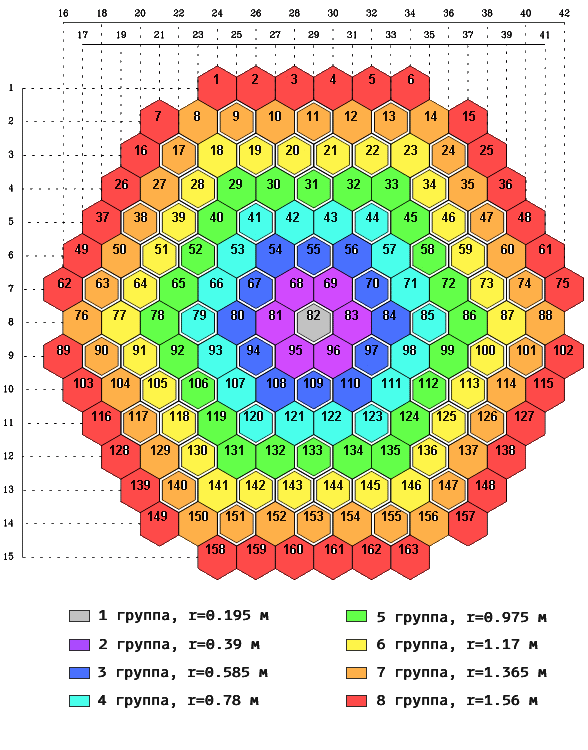
\includegraphics[scale=0.7]{treton_cells.png}
		\caption{Картограмма ячеек моделируемой АЗ для расчетного кода «ТРЕТОН» и их разбиение на группы по радиусу}
		\label{pic:treton-kartogramma}
	\end{center}
\end{figure}


Для каждой зоны были расчитаны тепловыделения, нормируя на соответствующие $K_r^i$, $K_z^j$, где $i = \overline{1, 8}$, $j = \overline {1, 30}$.

Распределение $K_r$ по группам было подобрано ориентируясь на следующие зависимости:
\begin{equation}
    K_r(r) \sim J_0(\frac{\xi_0 r}{R_{\text{эфф}}}) \approx - \alpha r^2 + \beta
\end{equation}, распределение коэффициента неравномерности по радиусу в приближении параболической функции
\begin{equation}
    \label{equation:KriNi}
    \sum_{i=1}^{8} K_r^i N_i = N_{\text{ТВС}} \pm 0.01
\end{equation}, где $N_i$ — количество ТВС в $i$-той группе по радиусу – условие нормировки распределения коэффициента неравномерности по радиусу.
Коэффициент $\beta$ параболической функции был подобран из условия, что в центре $K_r(r=0)$ должна быть равна табличному значению $K_r$ из \ref{tabular:data}, коэффициент $\alpha$ для удовлетворения соотношения \ref{equation:KriNi}. Полученные значения распределения коэффициента неравномерности по радиусу для каждой группы представлены в таблице \ref{tabular:Kri}.

\begin{figure}[H]
	\begin{center}
		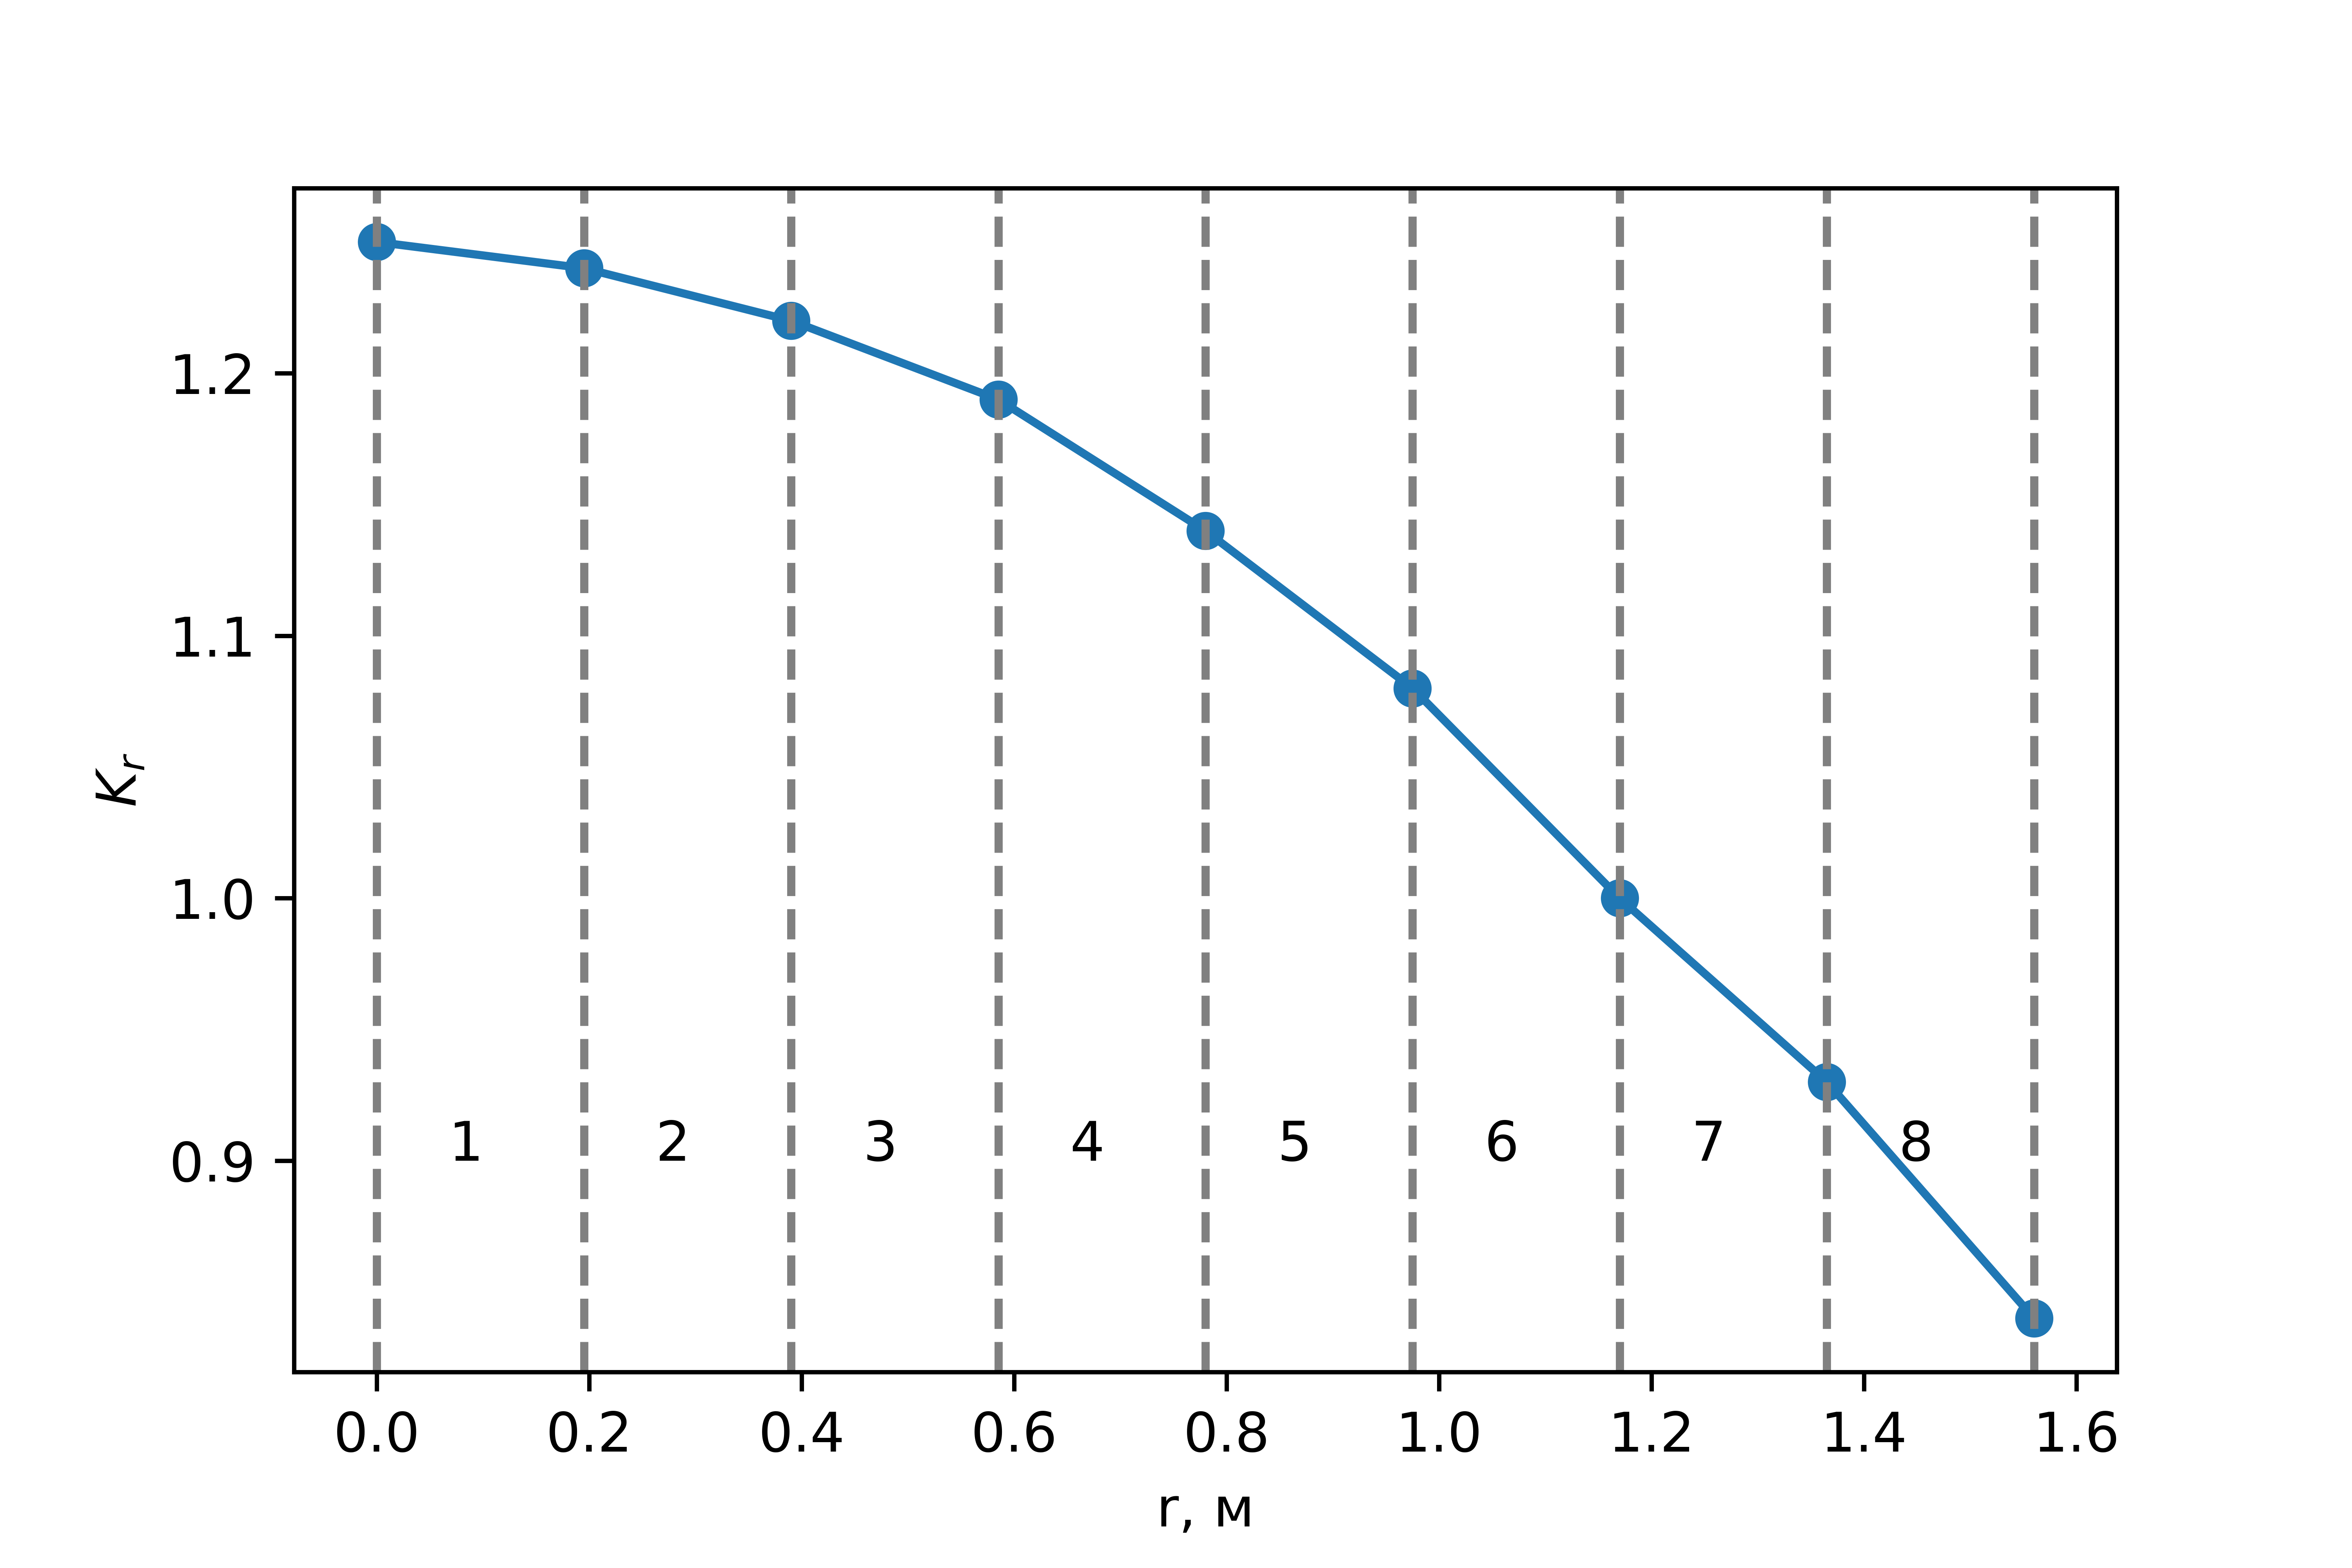
\includegraphics[scale=0.8]{Kr.png}
		\caption{Распределение коэффициента неравномерности по радиусу для восьми групп ТВС}
		\label{pic:Kr}
	\end{center}
\end{figure}

\begin{table}[H]
	\caption{Коэффициент неравномерности энерговыделения по радиусу для групп ТВС}
	\begin{center}
        \begin{tabular}{|l|c|}
        \toprule
         Номер группы & Значение $K_r^i$ \\
         \midrule
         \hline
         1 & 1.24 \\
         \hline
         2 & 1.22 \\
         \hline
         3 & 1.19 \\
         \hline
         4 & 1.14 \\
         \hline
         5 & 1.08 \\
         \hline
         6 & 1.00 \\
         \hline
         7 & 0.93 \\
         \hline
         8 & 0.84 \\
         \bottomrule
		\end{tabular}
		\label{tabular:Kri}
	\end{center}
\end{table}


\noindent Распределение коэффициента неравномерности по высоте $K_z$ определяется как:
\begin{equation}
    K_z(z) = K_z \cos \left( \frac {\pi z} {H_{\text{эфф}}} \right)
\end{equation}
где $z = \overline{-H_{\text{АЗ}} / 2,\  H_{\text{АЗ}} / 2}$ м.


\noindent Распределение $K_z$ по высоте представлено на рис \ref{pic:Kz}


\begin{figure}[H]
	\begin{center}
		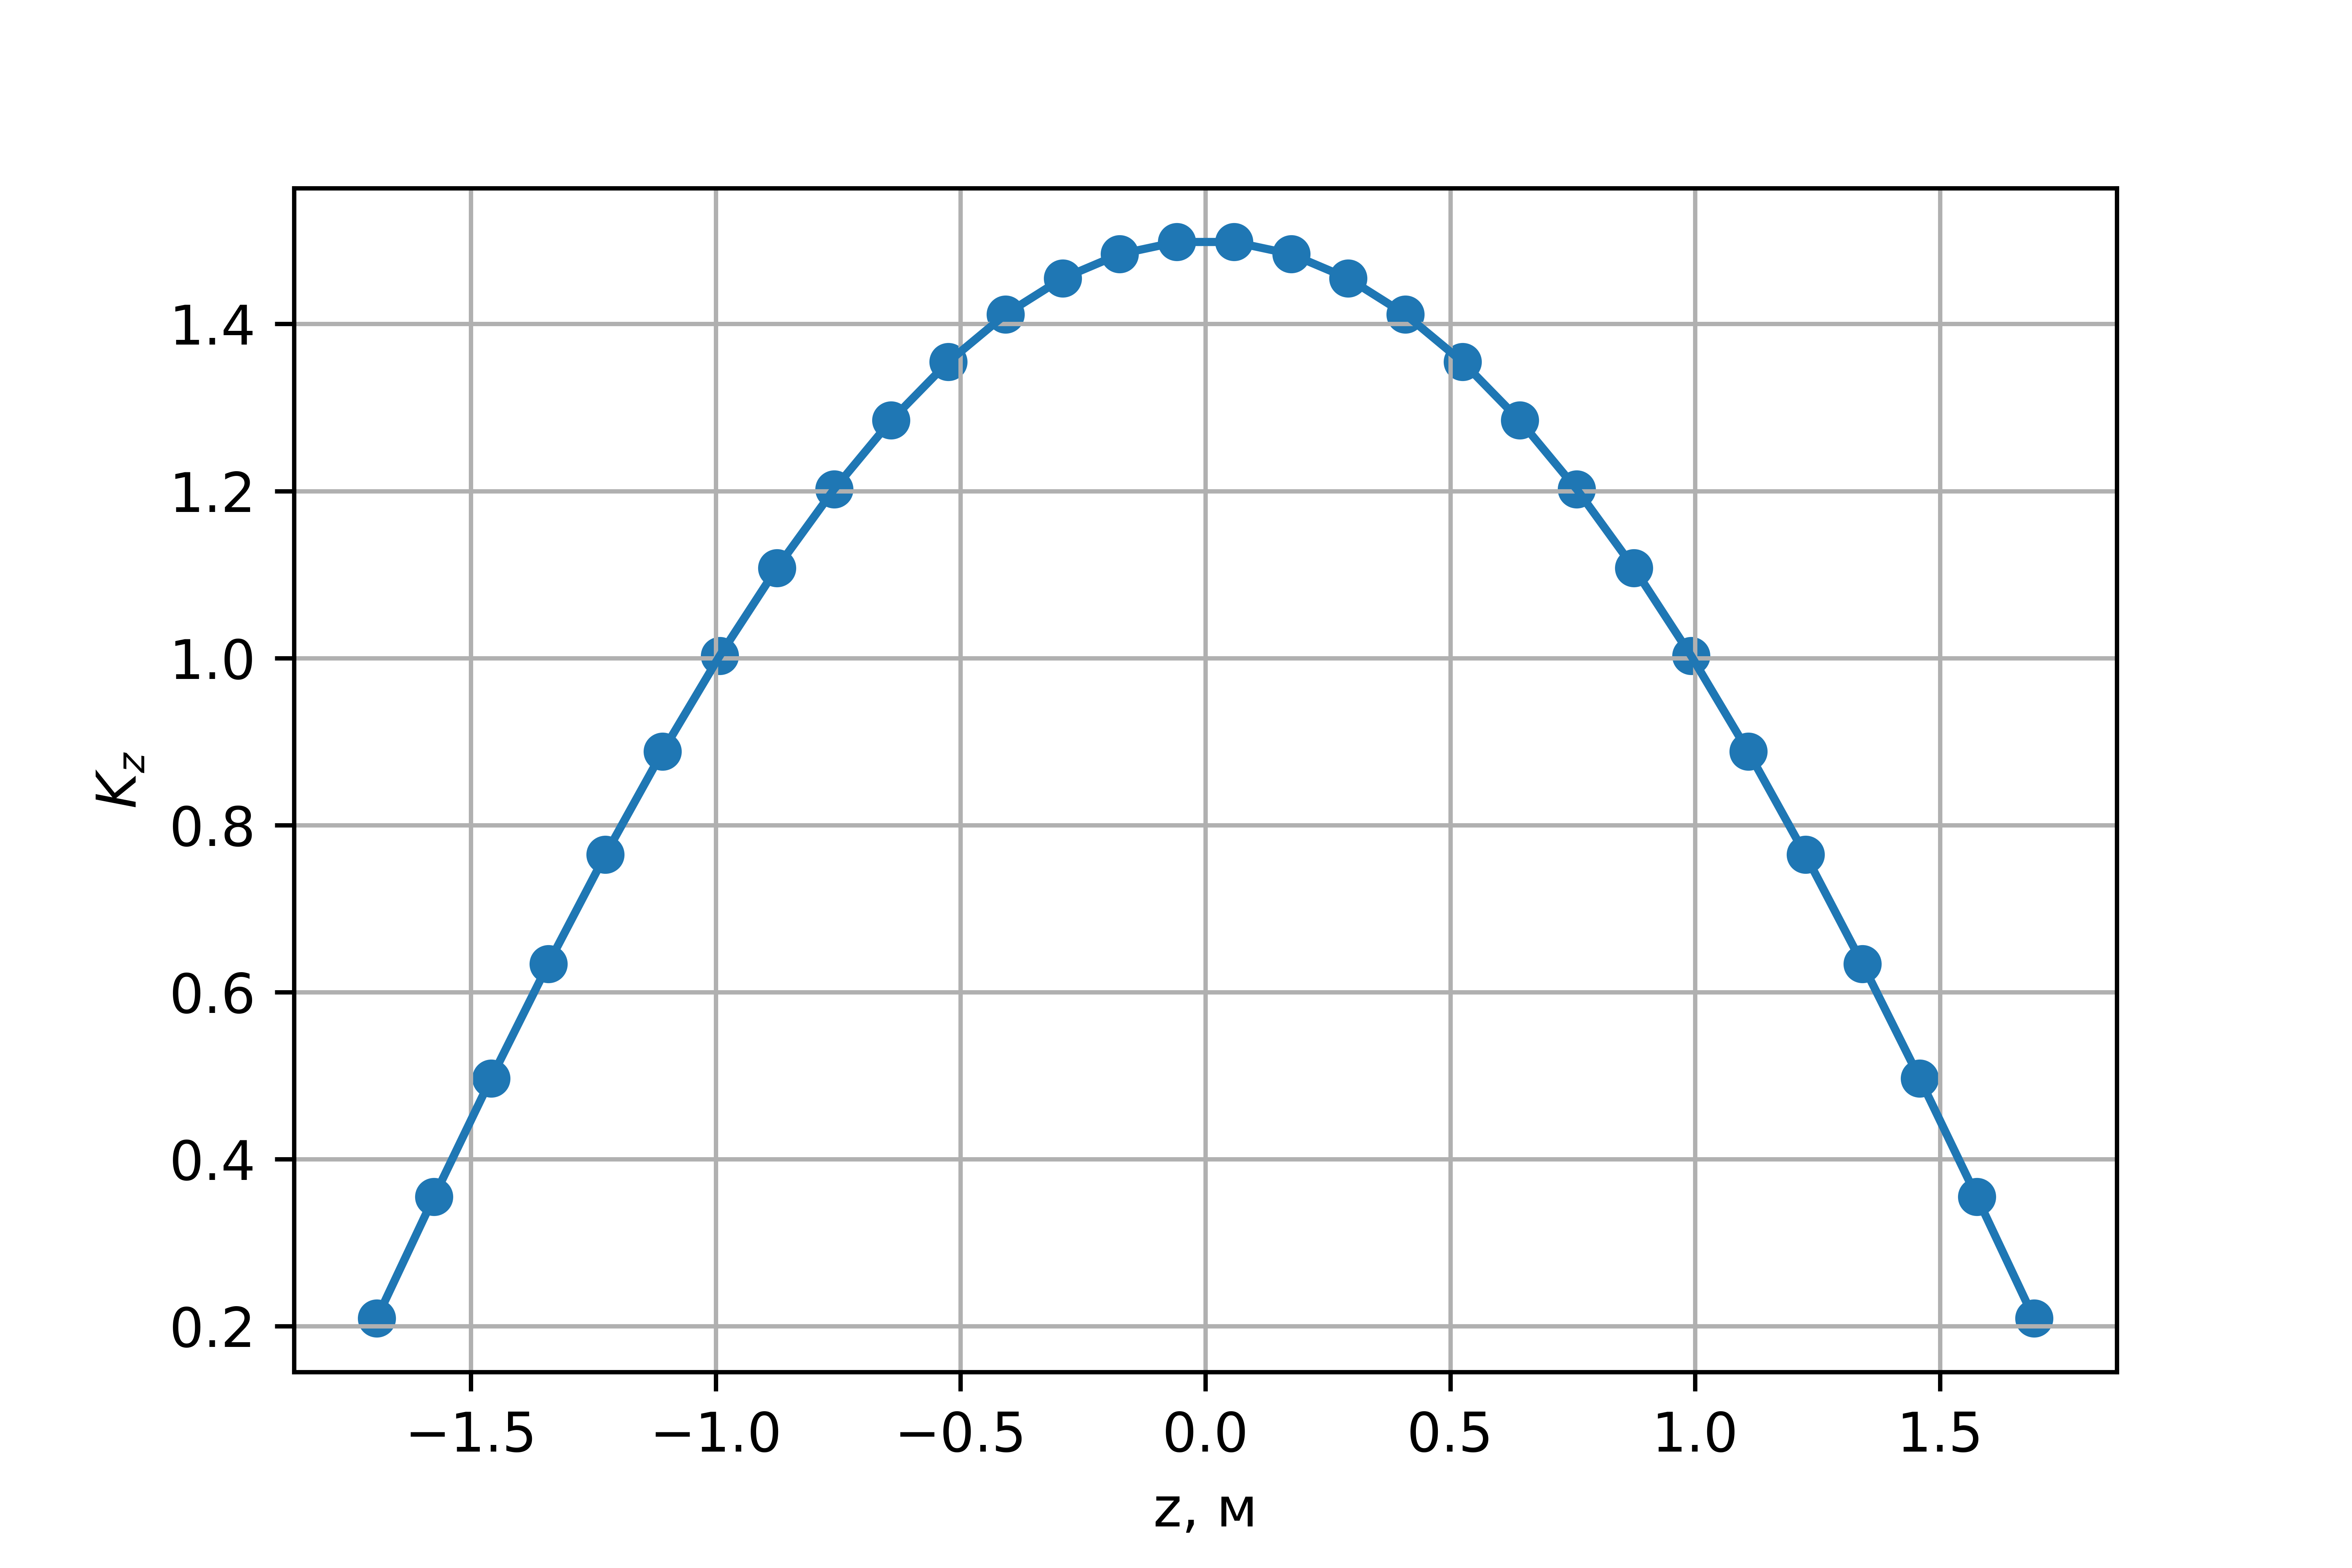
\includegraphics[scale=0.8]{Kz.png}
		\caption{Распределение коэффициента неравномерности по высоте активной зоны}
		\label{pic:Kz}
	\end{center}
\end{figure}


Из полученных распределений $K_r$, $K_z$ было определено распределение тепловыделения для всех групп расчетных элементов
\begin{align}
    \label{equation:Qzr}
    Q(z, r) &= K_z(z)K_r(r)\frac{Q_{\text{теп}}}{N_{\text{ТВС}} \cdot 30} \\
            &= K_r(r) K_z \cos \left( \frac{\pi z}{H_{\text{эфф}}} \right) \frac{Q_{\text{теп}}}{N_{\text{ТВС}} 30}
\end{align}

На основе соотношения \ref{equation:Qzr} был сформирован входной файл \texttt{Q6.txt} с тепловыделением для всех расчетных элементов в соответствии с картограммой \ref{pic:treton-kartogramma}

Далее были проведены калибровочные расчеты для определения входных параметров файла \texttt{THEHYCO.INI}, соответствующих проектируемой РУ. Основным критерием выбора параметров было соответсвие вычисленному программой «ТРЕТОН» расходу полученному ранее в рамках теплофизического расчета.

Таким образом расчетным кодом было получено значение расхода $G_{\text{расч}} = (1.570 \pm 0.016) \cdot 10^4\  \frac{\text{кг}}{\text{с}}$, что соответствует полученному ранее значению $G_{\text{реак}} = 1.579 \cdot 10^4\ \frac{\text{кг}}{\text{с}}$ в пределах погрешности. 
Значения входных параметров файла \texttt{THETHYCO.INI}, при которых достигнут такой расход приведены в таблице % \ref{tabular: thethyco_nominal}


% TODO: табличка с параметрами THEHYCO.INI по разделам с именами

% \begin{table}[H]
% 	\caption{wow}
% 	\begin{center}
%         \begin{tabular}{|l|c|}
%         \toprule
%          Раздел RodList & \\
%          \midrule
%          \hline
%          tmp=0.75 3.86 4.25 4.55 & разбиение твэлов на контрольные объемы, указаны радиусы центрального отверстия твэла, границы топливного столба, центра оболочки, внешней границы оболочки. мм\\
%          \hline
%          $\texttt{s_mesh}$=12.75 & шаг твэлов, мм \\
%          \hline
%          d\_mesh=9.1 & диаметр твэла, мм \\
%          \hline
%         %  $\texttt{R_contact}$=0.00024 & контактное сопротивление толиво-оболочка, $\text{м}^2 \cdot \text{К} / \text{Вт}$ \\
%         %  \hline
%          Раздел HEATandHYDROlist & \\
%          \midrule
%          \texttt{dr}=0.241 & поперечный размер расчетной области, м\\
%          \hline
%          \texttt{dz}=0.118 & продольный размер расчетной области, м\\
%          \hline
%          $\texttt{n_RodsInTVS}$ =317 & количество твэлов в ТВС \\
%          \hline
%          \texttt{Disbalance}=0.001 & расчетный дисбаланс \\
%          \hline
%          $\texttt{p_input}$=15800000 & входное давление, Па \\
%          \hline
%          $\texttt{p_output}$=15691054 & выходное давление,  Па \\
%          \bottomrule
% 		\end{tabular}
% 		\label{tabular:thehyco_nominal}
% 	\end{center}
% \end{table}

На основе описанных входных параметров был произведен расчет с шагом по времени $dt=0.0005$ для 100 итераций. По результату расчета были построены зависимости температур теплоносителя, внутренней, наружней стенки по высоте активной зоны для каждой группы а также для кассет, с максимальными температурами. Также были построены распределения подогревов плотность и расходы



% Не редактируем: Страница библиографии (формируется автоматически из книжек, указанных в refs.bib и пометок \cite{имя_источника} в тексте)
\include{templates/bibpage}
\end{document}
